\chapter{Integration of Non-Inclusive Contacts in Posture Generation}

\section{abstract}
In this paper we propose a simple way to formulate geometric contact formation to have an arbitrary intersection shape in a robotic (humanoid) posture generation problem. The contact shape is the outcome of our posture generator that is formulated as a non-linear optimization programming to fulfill a large variety of robot intrinsic limitations (e.g. joint and torque limits) and tasks (e.g. desired contact). Starting by defining convex areas of contact on the robot's body and the environment, that we call contact patches, we can generate contacts with arbitrary intersection of a pair of any of these predefined patches. Our geometric contact modeling writes very simply as additional constraints and variables added to the optimization problem, translating the search for an ellipse inscribed in the intersection of the pair of patches we want in contact. The result of our posture generator is then a configuration where contact patches are not necessarily included in one another. This allows our posture generator to propose contacts of different shapes with a non-predefined number of contact points (used later to compute reaction/contact forces). We illustrate the efficiency of our method in multi-contact posture generation with the HRP-2 and ATLAS humanoid robots with results that can not be generated automatically by existing methods.
%That is to say, the constraints formulating a new contact in the posture generator (that writes as a non-linear optimization problem), state that a surface is totally included into another. Moreover contact surfaces are modelled by four vertices only and are rectangular. This modelling has several limitations: (i) it excludes several viable solutions that the planar could exploit, (ii) it requires patching (by hand) the robot or the environment surfaces into somehow equivalent pieces of rectangles, (iii) do not allow singular contacts of type edge/plan (ladder) or rarely edge/edge and vertex/plan. The solution we provide solves this problem and extend our multi-contact planner possibilities to handle more complex scenarios without patching the robot or the environment surfaces and without limiting the number of contact points per surface of contact.


%%%%%%%%%%%%%%%%%%%%%%%%%%%%%%%%%%%%%%%%%%%%%%%%%%%%%%%%%%%%%%%%%%%%%%%%%%%%%%%%
\section{Introduction}
\label{sec:intro}

Generating viable robotic postures is a common problem encountered in sampling-based planning techniques and simulation of virtual characters. Generating desired initial, intermediary or finale posture configurations requires defining static task goals (e.g. reach a target point in 6D) to be done under intrinsic constraints such as joint limits, torque limits, avoiding non-desired self-collisions... and perceptual or extrinsic ones such as keeping an object in the embedded camera field-of-view, avoiding non-desired collisions with surrounding objects, etc. A common task objective assigned to virtual characters, avatars, or humanoid robots is to contact one or more of its links with the environment (e.g. feet touching the ground). Since our main applications target humanoid robots, we consider here posture generation problems inherent to these robots. However, the formalism applies to any kind of robots achieving contacts with its surroundings or itself.

Our problem is to generate multi-contact viable postures. As far as humanoids are concerned, we may add to the previously cited constraints, equilibrium and non-sliding. This paper is dedicated to the focused issue of how contact constraints can be written geometrically. Generating postures often uses state-of-the-art enhanced inverse kinematics or general-purpose non-linear optimization programming (where inverse kinematics can be seen as a particular solver case).  

%\begin{figure}
%\centering
%\begin{subfigure}{.5\columnwidth}
%  \centering
%  \setlength\fboxsep{0pt}
%  \setlength\fboxrule{1pt}
%  \fbox{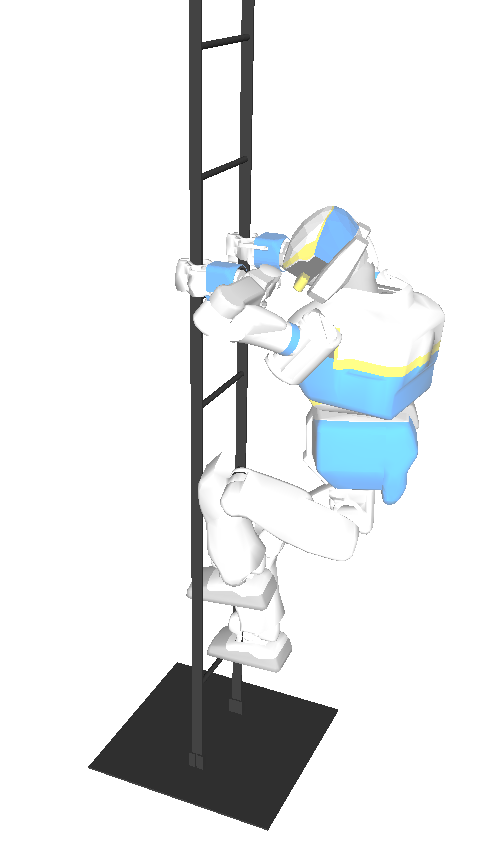
\includegraphics[width=\linewidth]{figure/hrp2_ladder_jrl.png}}
%  \label{fig:hrp2_jrl}
%\end{subfigure}%
%\begin{subfigure}{.5\columnwidth}
%  \centering
%  \setlength\fboxsep{0pt}
%  \setlength\fboxrule{1pt}
%  \fbox{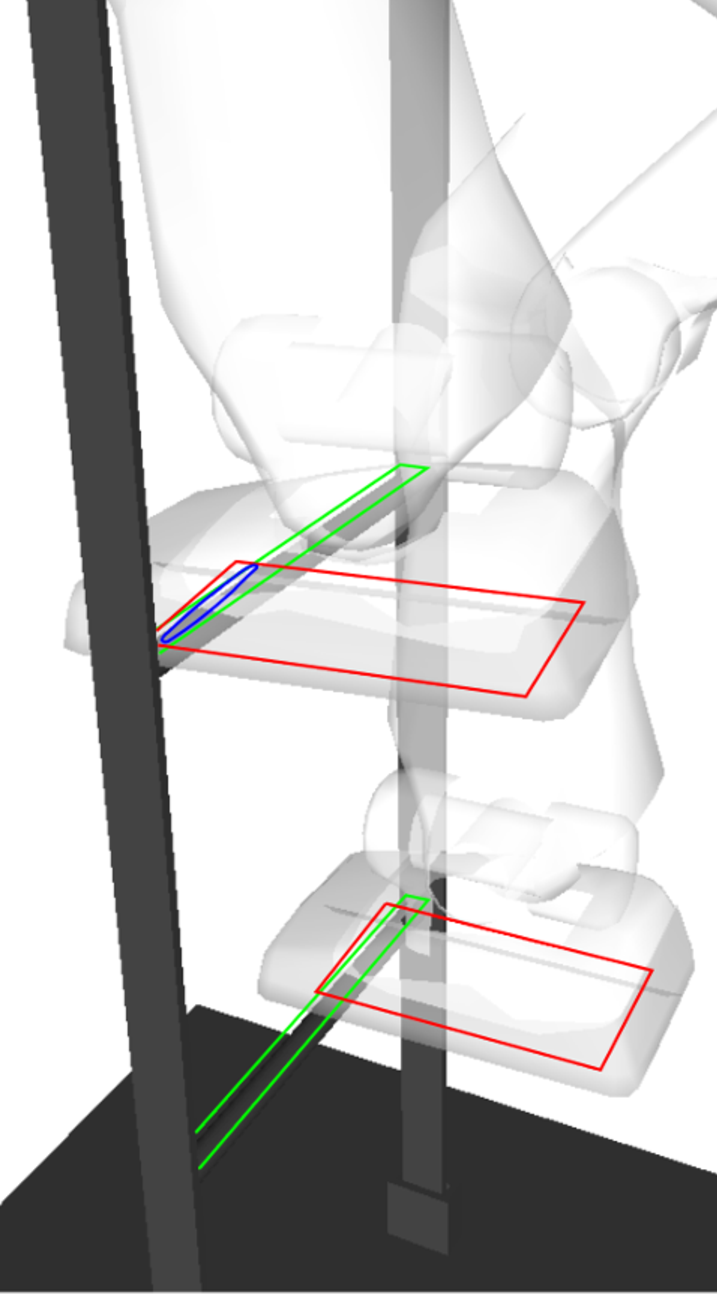
\includegraphics[width=\linewidth]{figure/hrp2_ladder_jrl_zoom.pdf}}
%  \label{fig:hrp2_jrl_zoom}
%\end{subfigure}
%\caption{Using non-inclusive contacts for ladder climbing\\(green/red: contact polygons; blue: contact ellipse)}
%\label{fig:hrp2_jrl_complete}
%\end{figure}  

\begin{figure}
\centering
  \centering
  \setlength\fboxsep{0pt}
  \setlength\fboxrule{1pt}
  \fbox{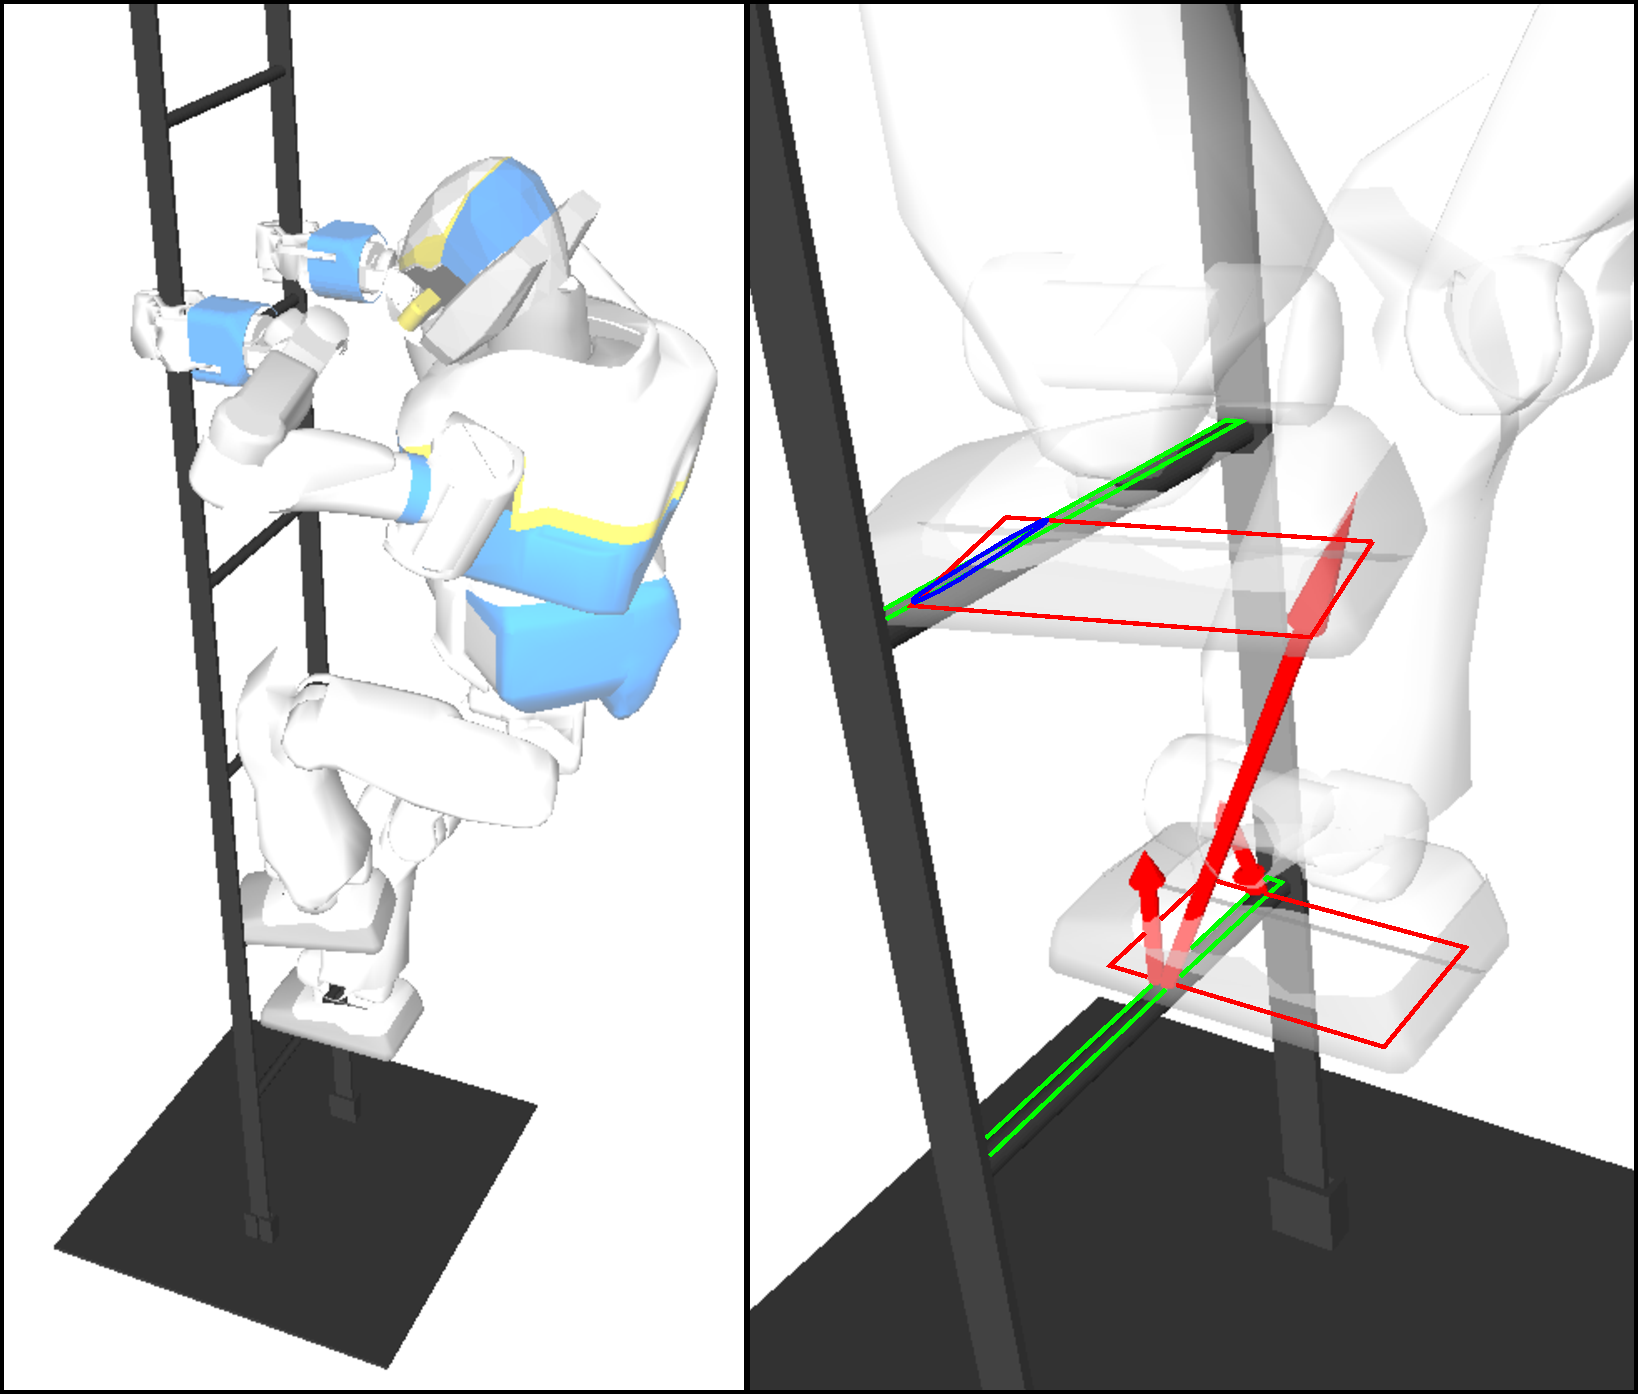
\includegraphics[width=.95\linewidth]{papers/IROS2014/figure/hrp2_ladder_jrl_5_combo.pdf}}
\caption{Using non-inclusive contacts for ladder climbing (green/red: contact polygons; blue: contact ellipse; red arrows: contact forces resultants)}
\label{fig:hrp2_jrl_complete}
\end{figure}  

In general, desired contacts write as hard constraints to fulfill in an optimization problem. Yet, we need to write the maths for, say, put the gripper on the wall and the left foot on the ground. In general, the maths of a gripper is a complex geometric description, so is often that of the environment. A contact is generally defined by a pair of points (one on each object in contact) and a pair of normal vectors. A hard contact constraint boils down to finding a posture in which the predefined authorized contact points and normal of each body match~\cite{zhang:TePRA:2013}\cite{hauser:IJRR:2008}. Likewise, in~\cite{osswald:iros:2011}, the position of the feet of the NAO robot is manually tuned in order to obtain statically stable position during the climbing of a spiral staircase. In~\cite{Chestnutt:2009:BNR:1733023.1733314}, the surface in contact is chosen according to two criteria: the position of the force sensors of the feet, and the type of contact desired. In~\cite{sentis:itro:2010}, the problem of contact discovery in not considered. In~\cite{mordatch:acm:2012}, two surfaces are considered in contact as soon as the center point of one of them touches the other one and their normals match. Although used in many papers, it is not difficult to see that this definition of contact excludes a series of possibilities that would have been obtained if the predefined points were placed in different configurations within their respective patches. Once the contact is established, one determines the intersection of contacting surfaces in order to find points on which reaction forces are to be computed. Several approaches require fixing the number of contact points or to have inclusive contact (i.e. one patch is fully included in the other)~\cite{bouyarmane:ar:2012}.

We provide a simple solution that relaxes hard contact constraints and gets rid of predefining the contact points by allowing them to travel within the patches. We consider that a contact is valid if the intersection between two distinct patches has an area greater than a given threshold. To enforce this, we require this intersection to contain an ellipse whose surface can possibly be maximized. Convex patches allow writing the inscription constraints easily by means of half-spaces. We finally implement our solution and present some examples for complex multi-contact posture generations with the HRP-2 and ATLAS robots, as shown in~\Figref{fig:hrp2_jrl_complete}. 


\section{Contact geometry formulation}

For our formulation, we consider a situation where a set of contacts between the robot and its environment are already made, and therefore fixed, and we want to add a new contact to this set. This doesn't induce any loss of generality since it just comes down to adding the contacts one by one.
To ensure that the new contact can be reached in a quasi-static way, we look for a configuration where the new contact is ``barely" made: the position of contact is reached, but that contact does not support any contact forces (this is a necessary step to generate a sequence of quasi-static transitions). We call it a geometric contact. Let us consider that the contact to add is defined by two flat surfaces $S_1$ and $S_2$ which are respectively delimited by two convex polygons $P_1$ and $P_2$. For this contact to be valid, it is obviously necessary that the intersection $P_1 \cap P_2$ is not empty. We propose a method in which the size of the contact area is approximated by the size of an ellipse that is inscribed in it. If such an ellipse is found and is of a sufficient size, then the contact is valid. This allows to consider contacts between surfaces that do not necessarily include each other.

An important remark is that the number of sides of the intersection polygon is not known a priori and, as shown on~\Figref{fig:polygon-inter}{}, this number can change depending on the configuration. Each time this number changes, the gradient of the area of the intersection is discontinuous. This is an issue for integrating any constraint or objective based on the area because we use a solver for smooth optimization problems. This issue could be dealt with by using non-smooth optimization routines, but such algorithms are slower and less available, and our posture generator is not designed to use them.
\begin{figure}[!htb]
 \centering
 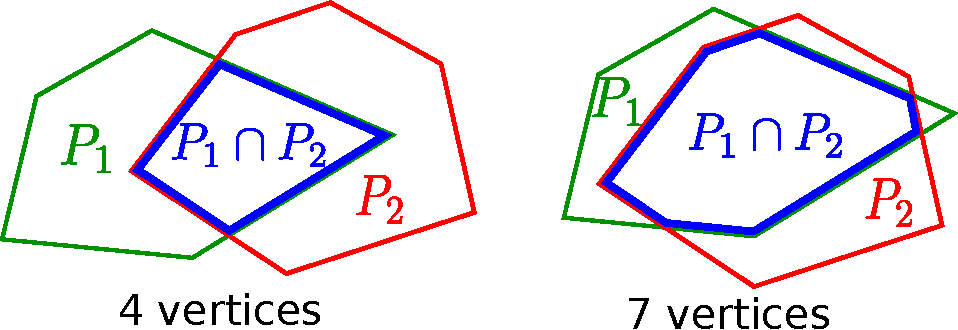
\includegraphics[width=0.8\columnwidth]{papers/IROS2014/figure/polygon-inter.pdf}
 \caption{Topological instability of $P_1 \cap P_2$}
 \label{fig:polygon-inter}
\end{figure}
Moreover, supposing that we want to write constraints based on the sides of the contact area, then, the number of constraints would change with the number of vertex of $P_1 \cap P_2$. The large majority of the optimization softwares cannot deal with a non-constant number of constraints. The solution proposed in section~\ref{sec:ellipse} overcomes these issues by defining a set of constraints that is independent from the topology of the intersection area.

\section{Posture generation}
\label{sec:pg}

The posture generation process aims at finding a posture that satisfies a set of tasks $\left\{ \mathcal{T}_i \right\}$ and that minimizes a cost function $\mbox{\emph{Cost}}$ by solving the following problem:
\begin{align}
\min_{\bf q, \bf f, \tau} & \quad \mbox{\emph{Cost}}({\bf q,f,\tau}) \nonumber\\
\text{s.t.}&
\left\{
\begin{array}{lr}
q_i^- \le q_i \le q_i^+\ \ \forall i=1,...,n \\
\tau_i^- \le \tau_i \le \tau_i^+\ \ \forall i=1,...,n \\
\epsilon_{ij} \le d(r_i({\bf q}), r_j({\bf q})),\ \ \forall(i,j)\in\mathcal{I}_{auto} \\
\epsilon_{ik} \le d(r_i({\bf q}, O_k)),\ \ \forall(i,k)\in\mathcal{I}_{coll}\\
\tau + J({\bf q})^T{\bf f} = {\bf g(q)}\\
s({\bf q,f})\le 0,\\
g_i({\bf q,f,\tau}) = 0\ \ \forall\mathcal{T}_i,\\
h_i({\bf q,f,\tau}) \le 0\ \ \forall\mathcal{T}_i.
\end{array}\right.
\label{eq:PG}
\end{align}
where the optimization variables $\bf q$, $\bf f$ and $\tau$ stand for the configuration, contact forces and joint torques of the robot.
Those constraints are illustrated in~\Figref{fig:PG}{} and are, in order of appearance:
\begin{itemize}
\item Joint limits
\item Torque limits
\item Auto-collisions, with $d(X,Y)$ the signed distance between objects $X$ and $Y$ and $r_i(\bf q)$ is the i-th body of the robot at configuration $\bf q$. $\mathcal{I}_{auto}$ is the set of pairs of bodies to monitor.
\item Collisions with the environment, $O_k$ being the k-th object in the environment and $\mathcal{I}_{coll}$ the set of pairs to monitor
\item Equation of static stability, with $J$ the Jacobian matrix of all points where the contact forces are applied, and $\bf g$ the gravity term.
\item Stability constraints describing the friction cones
\item Equality constraints describing the task $\mathcal{T}_i$
\item Inequality constraints describing the task $\mathcal{T}_i$
\end{itemize}

\begin{figure}[!htb]
 \centering
 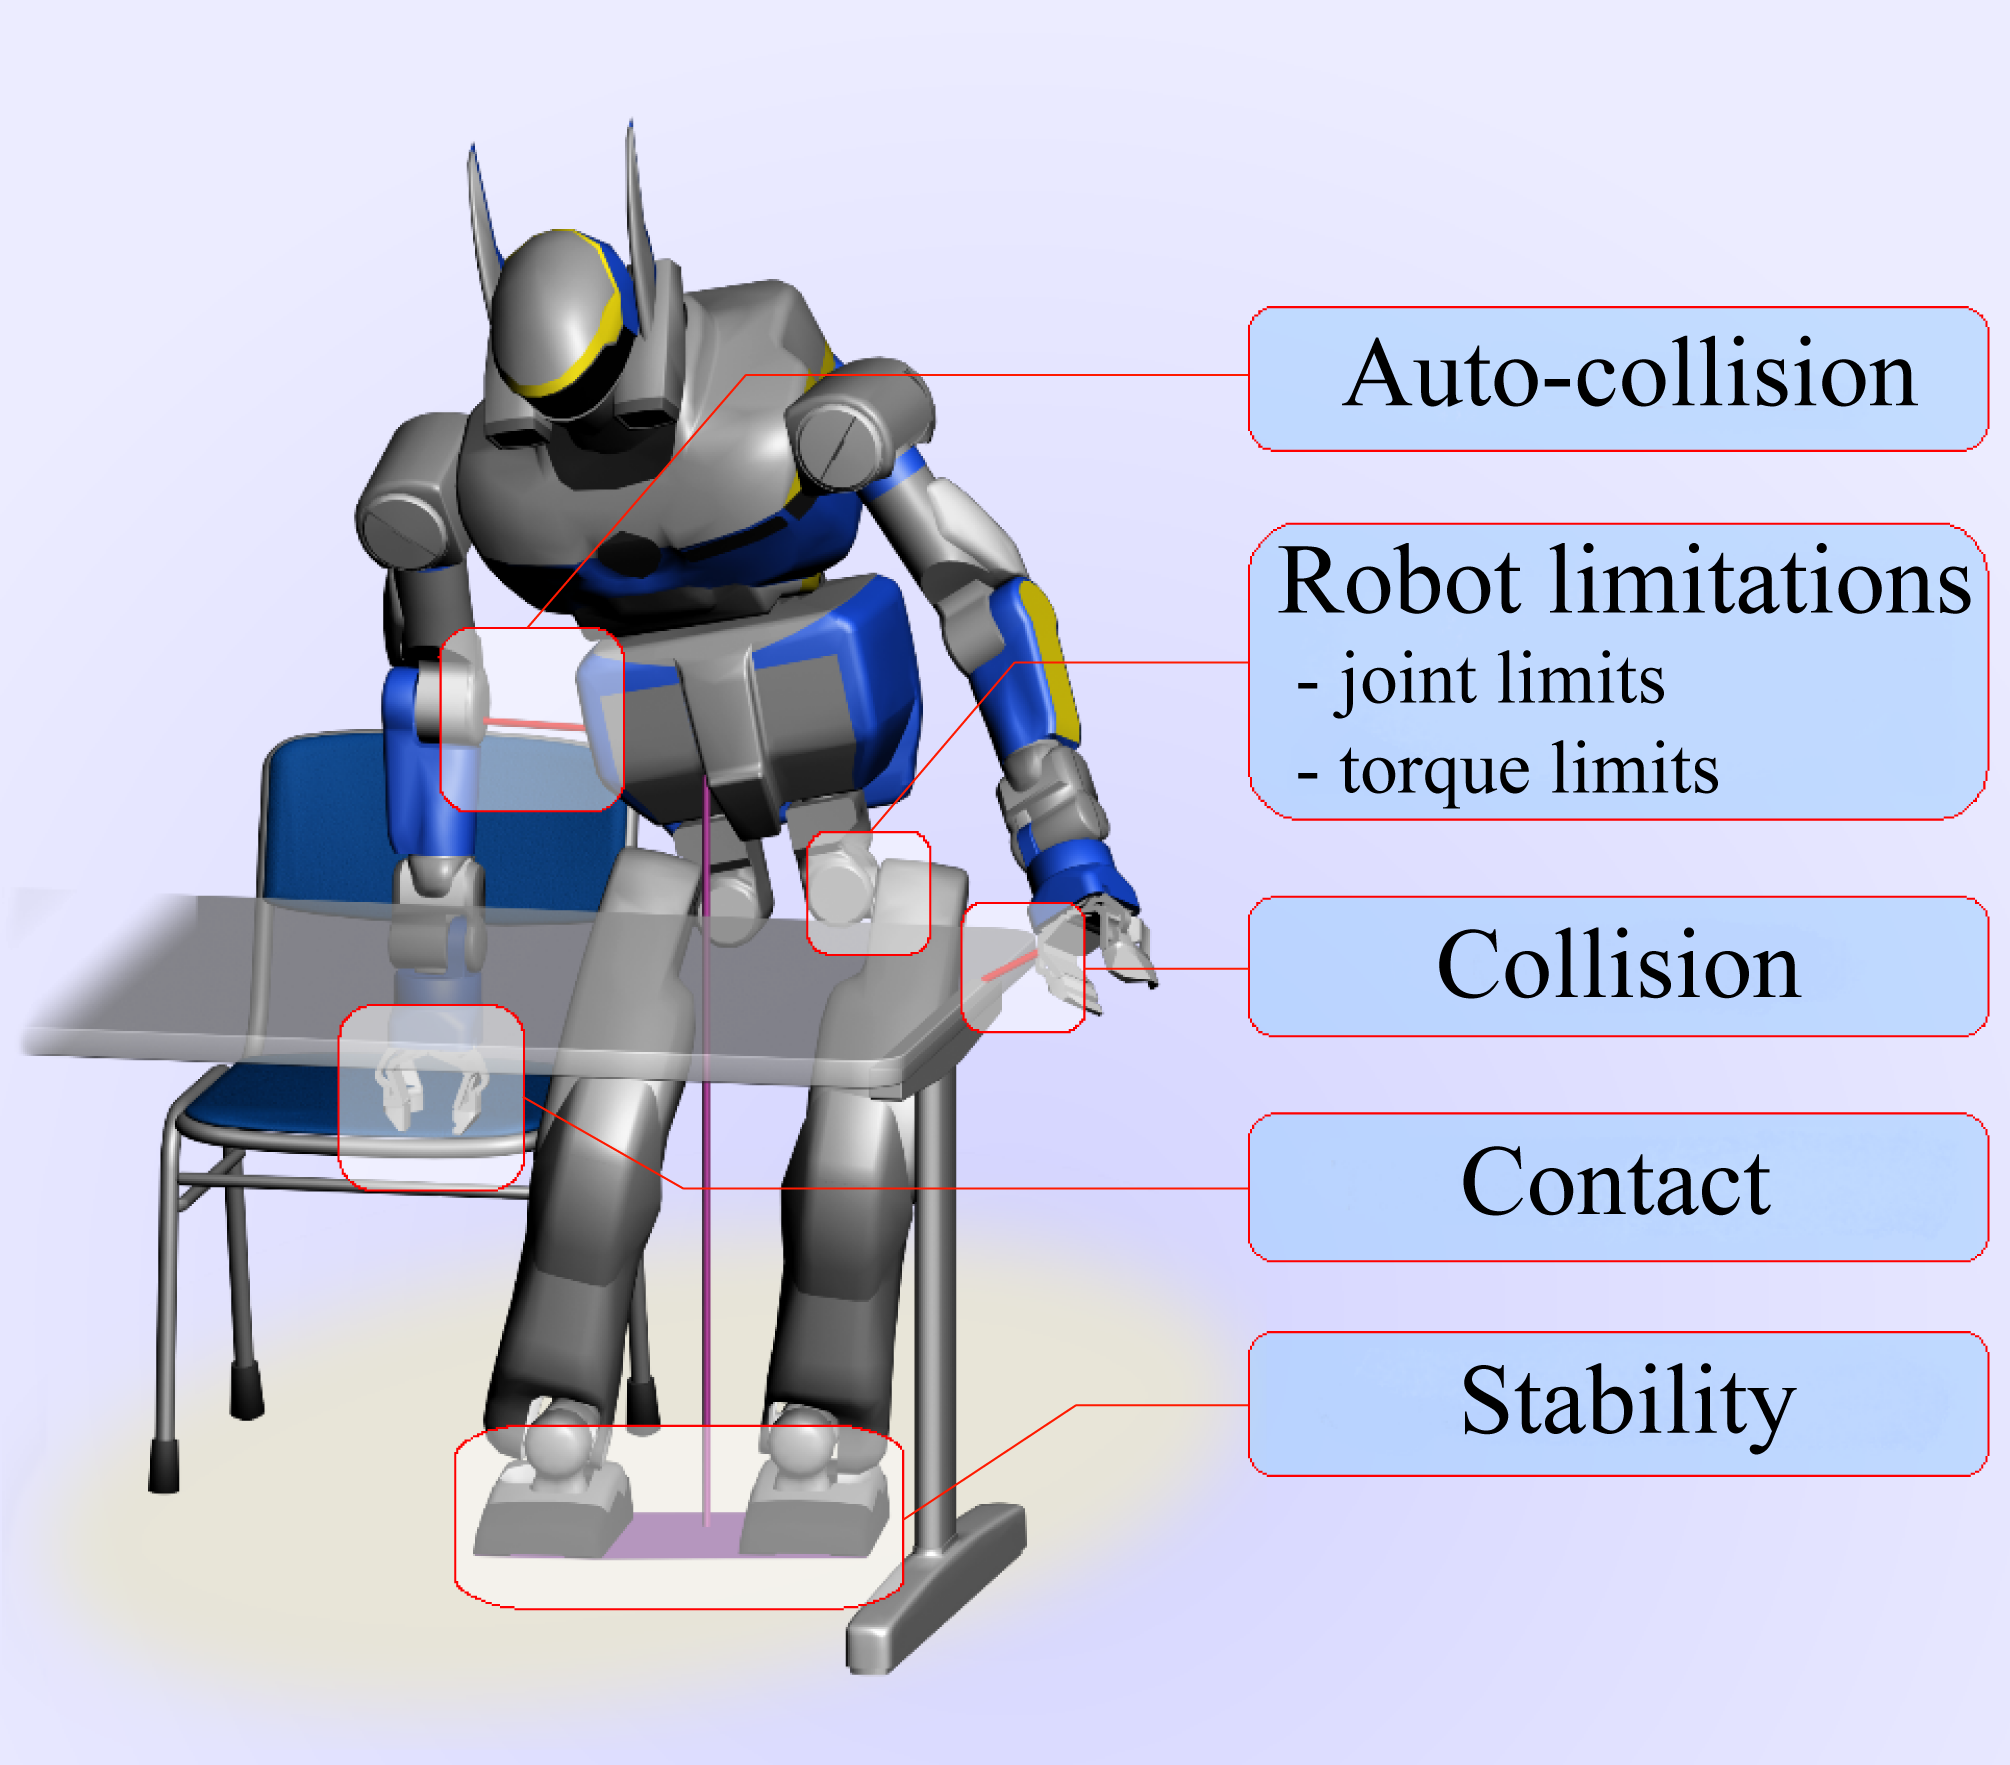
\includegraphics[width=.9\linewidth]{papers/IROS2014/figure/PG.png}
 \caption{Posture Generation's usual constraints}
 \label{fig:PG}
\end{figure}

A usual task $\mathcal{T}_i$ in the posture generation is to ensure that two surfaces are in contact. We consider 2 polygons $P_1$ and $P_2$ described in 2 frames $\mathcal{F}_1$ and $\mathcal{F}_2$, respectively. Each frame is defined by an origin point ${\bf O_i} = (o_i^x, o_i^y, o_i^z)$ and 3 orthogonal vectors $[{\bf T_i, B_i, N_i}]$. In those frames, the polygons are described as a set of $n_i$ bi-dimensional points $[p_i^0, p_i^1,\ldots, p_i^{n_i-1}]$ lying in the $[{\bf O_i, T_i, B_i}]$ plane.
To ensure the contact between those two surfaces, it is necessary that the planes defined by $[{\bf O_1, T_1, B_1}]$ and $[{\bf O_2, T_2, B_2}]$ are coplanar. This is expressed by the set of equations~(\ref{eq:coplanarity}). Those equations define a floating contact, where the co-planarity is ensured and the surfaces can translate along $\bf T_1$ and $\bf B_1$ and rotate around $\bf N_1$.
\begin{equation}
\left\{
\begin{array}{lr}
{\bf (O_2-O_1).N_1} = 0 \\
{\bf T_2.N_1} = 0 \\
{\bf B_2.N_1} = 0 \\
{\bf -N_2.N_1} \le 0
\end{array}
\right.
\label{eq:coplanarity}
\end{equation}

However, this is not sufficient since nothing ensures that the intersection of $P_1$ and $P_2$ is not empty.
Up to now, to avoid the problems described in section~\ref{sec:background}, we were requiring that one of the two polygons was completely included into the other (which restricted the contact configuration possibilities) or by defining a fixed contact position by hand, in which case the non-emptiness is ensured by the user. The next section presents a more general formulation
%The inclusion of the polygon $P_i$ in the polygon $P_j$ is imposed by making sure that each vertex of $P_i$ is on the left side of every edge of $P_j$, that is, assuming that both polyg polygonsons are described counter-clockwise around the ${\bf N}$ vector of the frame to which they are attached, the algorithm \ref{alg:inclusion} summarizes that constraint.
%\begin {algorithm}
%\caption{Surface inclusion constraints for $S_i \subset S_j$}
%\begin{algorithmic}
%\STATE {Let $S_i$ and $S_j$ be two coplanar plane surfaces}
%\STATE {$S_i = {p_0, p_1, \ldots, p_n}$ and $S_j = {q_0, q_1, \ldots, q_m}$}
%\STATE {$\vec{N}$ is $S_i$'s normal vector}
%\FOR{$k = 0 \to n$}
%\FOR{$l = 0 \to m$}
%\STATE { Constraint $: %\left[\overrightarrow{q_lp_k}\times\overrightarrow{q_lq_{l+1}}\right].\vec{N} \leq 0$}
%\ENDFOR
%\ENDFOR
%\end{algorithmic}
%\label{alg:inclusion}
%\end{algorithm}

\section{Non inclusive contact constraints}
\label{sec:ellipse}
\subsection{Main Idea}
\label{subsec:idea}
We present our main contribution: a smooth formulation of the non empty intersection between two contact surfaces. We assume that co-planarity of $S_1$ and $S_2$ is obtained by using the constraints presented in the previous section. Here we focus on the intersection of the two polygons $P_1$ and $P_2$, respectively describing the contours of $S_1$ and $S_2$.
As we pointed out earlier, a problem with computing the area of intersection of two polygons comes from the fact that depending on their positions in space, the number of edges of their intersection can change (cf.~\Figref{fig:polygon-inter}{}), which induces discontinuity of the gradient of the area and change of the number of constraints associated with this contact.

To avoid dealing with these changes of topology, we consider using an ellipse $\mathcal{E}$ included in $P_1 \cap P_2$ to estimate the area of the intersection. Since $P_1$ and $P_2$ are convex polygons, then $P_1 \cap P_2$ is also a convex polygon. A convex polygon can be seen as an intersection of half-planes based on the lines supporting its edges. Thus, an ellipse is inside a convex polygon if it lies entirely in the corresponding half-planes. Having the ellipse be included in the intersection of two polygons is equivalent to having it included in both polygons:
\begin{equation}
\mathcal{E} \subset P_1 \cap P_2 \ \Longleftrightarrow \ 
\mathcal{E} \subset P_1 \ \ \wedge \ \  \mathcal{E} \subset P_2
\end{equation}
Even if the number of edges of $P_1 \cap P_2$ can change, the numbers of edges of $P_1$ and $P_2$ respectively are fixed. 
%\begin{wrapfigure}{r}{0.4\columnwidth}
%  \begin{center}
%    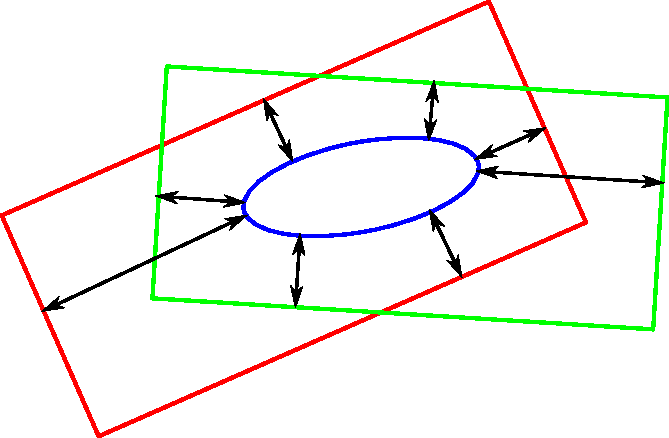
\includegraphics[width=0.4\columnwidth]{papers/IROS2014/figure/distance.pdf}
%    \caption{Distance ellipse-polygons}  
%  \end{center}
%  \label{fig:distance}
%\end{wrapfigure}
%Therefore, if we ensure that the ellipse $\mathcal{E}$ is on the left side of each segment defining $P_1$ and $P_2$, then it is inside $P_1 \cap P_2$. 
To assert that an ellipse lies in a half-plane, we need a function that is positive when the ellipse is in it (with zero value when the ellipse is on the edge) and negative if not. The signed distance to the line defining the half-space is a good candidate (distance ellipse-line if the ellipse is in the half-plane, opposite of the penetration distance if not), but actually, any pseudo-distance does the job. And a sufficient condition for the ellipse to be inside the polygons intersection is that the pseudo-distance between the ellipse and each edge of both polygons is positive (see~\Figref{fig:distance}{}). By considering each edge separately as opposed to the (pseudo-)distance of the ellipse to a whole polygon, we can write smooth constraints with a simple pseudo-distance function. We develop such a pseudo-distance in the next subsection. 
%In order to measure the fact that a point is on the left side of an oriented segment we use a signed distance $d_s$, this signed distance is positive and equal to a usual distance when the point is on the left side of the segment and is negative and equal to the opposite of the usual distance when the point is on the right side of the segment. 
% and algorithm~\ref{alg:ellipse-in-intersection} where $d_s$ stand for the pseudo-distance.
%\begin {algorithm}
%\caption{Inclusion of ellipse $\mathcal{E}$ in polygon intersection}
%\begin{algorithmic}
%\STATE {Let $P_1$ and $P_2$ be two coplanar convex polygons}
%\STATE {Let {\bf V} be an empty vector}
%\FORALL{Edge E in $P_1$}
%\STATE {Add $d_s(\mathcal{E}, E)$ to {\bf V}}
%\ENDFOR
%\FORALL{Edge E in $P_2$}
%\STATE {Add $d_s(\mathcal{E}, E)$ to {\bf V}}
%\ENDFOR
%\IF {{\bf V}$\succ 0$ (all terms of {\bf V} are positive)}
%\STATE {Return $\mathcal{E} \subset P_1 \cap P_2$}
%\ELSE
%\STATE {Return $\mathcal{E} \not\subset P_1 \cap P_2$}
%\ENDIF
%\end{algorithmic}
%\label{alg:ellipse-in-intersection}
%\end{algorithm}
%
\begin{figure}[!htb]
 \centering
 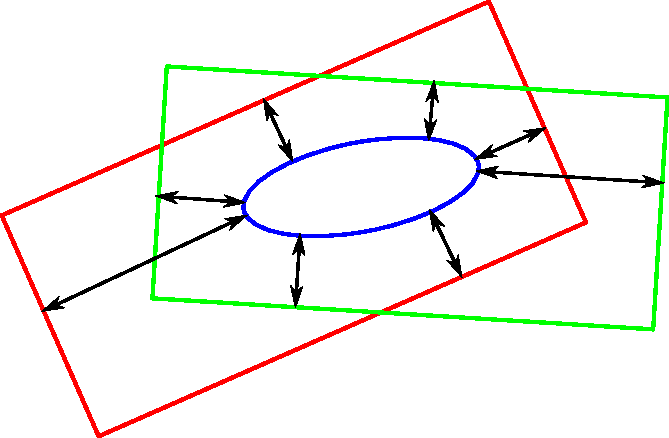
\includegraphics[width=0.4\columnwidth]{papers/IROS2014/figure/distance.pdf}
 \caption{Distance between $\mathcal{E}$ and $P_1 \cap P_2$}
 \label{fig:distance}
\end{figure}

\subsection{Pseudo-distance}
\label{subsec:formulation}
To estimate the constraint of inclusion of the ellipse $\mathcal{E}$ in both polygons $P_1$ and $P_2$, we need to compute the signed distance between $\mathcal{E}$ and each segment of the polygons. Computing the distance between an ellipse and a line is not straightforward, whereas the distance between a line and a circle is very easy to compute. Also, we note that in the frame $F_\mathcal{E}$ defined by the ellipse's axes and pseudo-radius, the ellipse is a circle of radius $r_{\mathcal{E}}=1$ (The x-unit along the first axis of the ellipse is $r_x$, the first radius of the ellipse, the y-unit along the second axis of the ellipse is $r_y$, the second radius). The transformation from the original frame $F_0$ in which the ellipse and the polygons are described to the ellipse's frame $F_\mathcal{E}$ is just the composition of a rotation and a scaling of the space along the axes of the ellipse with a scaling vector $[\frac{1}{r_x}, \frac{1}{r_y}]$. The effect of such a transformation applied to an ellipse and two polygons is shown in~\Figref{fig:pseudo-distance}{}. %Also, those transformations will not modify the validity of our constraint, indeed, the distance between $\mathcal{E}$ and any segment $E$, computed in $F_\mathcal{E}$, is a pseudo-distance in $F_0$. Therefore, we still get all the information needed to ensure the inclusion of $\mathcal{E}$ in $P_1 \cap P_2$.
We thus defined the following pseudo-distance from an ellipse to a half-plane as the signed Euclidean distance from the corresponding unit circle to the transformed half-plane in the frame $F_\mathcal{E}$.

\begin{figure}[!htb]
 \centering
 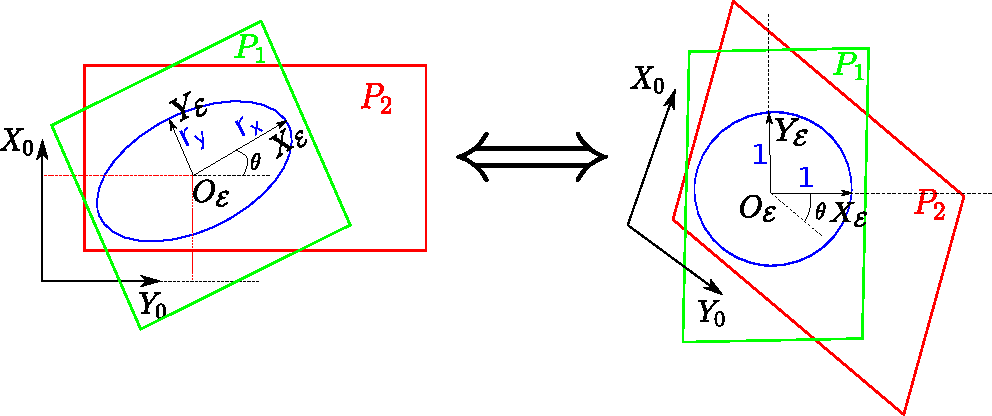
\includegraphics[width=\linewidth]{papers/IROS2014/figure/pseudo-distance.pdf}
 \caption{Transformation from $F_0(O_0, X_0, Y_0)$ to $F_\mathcal{E}(O_\mathcal{E},X_\mathcal{E},Y_\mathcal{E})$}
 \label{fig:pseudo-distance}
\end{figure}

Now let us consider a single segment $p_i p_j$ and an ellipse $\mathcal{E}$ defined in $F_0$.
The expression of a vector ${\bf v}_{F_0}^T = [v_x, v_y]_{F_0}$ in $F_\mathcal{E}$ is obtained by applying the formula~(\ref{eq:F0-to-FE})
\begin{equation}
{\bf v}_{F_\mathcal{E}} =
\begin{pmatrix}
\frac{1}{r_x} & 0 \\
0 & \frac{1}{r_y}
\end{pmatrix}
.\begin{pmatrix}
\cos(\theta) & \sin(\theta) \\
-\sin(\theta) & \cos(\theta)
\end{pmatrix}
.{\bf v}_{F_0}
\label{eq:F0-to-FE}
\end{equation}
In $F_\mathcal{E}$, the distance between the circumference of $\mathcal{E}$ and the segment $p_i p_j$ is: 
\begin{equation}
	d_s(\mathcal{E}, p_i p_j) = \frac{ \left(\overrightarrow{p_i p_j}\right)_{F_\mathcal{E}} \times \left(\overrightarrow{p_i O_\mathcal{E}}\right)_{F_\mathcal{E}}}{\| \overrightarrow{p_i p_j}\|_{F_\mathcal{E}}}-r_{\mathcal{E}}
\end{equation}
where $\times$ denotes the cross product and $O_{\mathcal{E}}$ is the center of the ellipse.

To avoid numerical problems when the segment $p_i p_j$ is small, (see sec.~\ref{subsec:singular cases}), it is preferable to multiply this distance by $\| \overrightarrow{p_i p_j}\|_{F_\mathcal{E}}$ before using it as a constraint. Then we get the following constraint: 
\begin{equation}
	-\left(\overrightarrow{p_i p_j}\right)_{F_\mathcal{E}} \times \left(\overrightarrow{p_i O_\mathcal{E}}\right)_{F_\mathcal{E}}+\| \overrightarrow{p_i p_j}\|_{F_\mathcal{E}} r_{\mathcal{E}} \leq 0
\label{eq:pseudo-distance}
\end{equation}

The combination of these equations~(\ref{eq:F0-to-FE}) and (\ref{eq:pseudo-distance}) applied for each edge of the polygons gives us all the necessary tools to develop a set of constraints that ensures that an ellipse is in the intersection of two polygons.


\subsection{Modification of the optimization problem}
To include the above idea in our posture generation, we need to modify the optimization problem~(\ref{eq:PG}) as follows.
Each non inclusive geometrical contact adds five variables to the optimization vector, corresponding to the position, orientation and radiuses of the ellipse ($x$, $y$, $\theta$, $r_x$ and $r_y$). One constraint of ellipse inclusion (as described above) is added to the problem for each edge of the polygons. The parameters $r_x$ and $r_y$ are given lower positive bounds to ensure that the ellipse is not empty. The existence of a contact between $S_1$ and $S_2$ is thus transformed into the existence of $r_x$ and $r_y$ respecting their bounds.
In summary, this kind of constraint adds 5 variables and $card(P_1)+card(P_2)$ constraints to the optimization problem, while the ``usual" inclusion constraint adds 0 variable and $card(P_1)card(P_2)$ constraints.
The existence of the contact can alternatively be enforced by imposing a minimum area for the ellipse.

\subsection{Maximization of the contact area}
\label{subsec:optim-ellipse-area}

%The previous section showed how to write a constraint describing the inclusion on any ellipse in the intersection of polygons. But it does not guarantee anything about the size of this ellipse nor about the size of the contact area. 
The formulation in the above section only ensures the existence of a contact of minimal size.
However, one could want to make sure to find a contact area as large as possible, so that it is more likely to be able to support strong forces and ensure strong friction forces, which is helpful to ensure the stability of the robot. Therefore, it seems appropriate to try and maximize the area of contact between two polygons. As explained before, computing the area of the intersection surface is not a good practice in our case. But we know that the ellipse computed as above gives a lower bound of the contact area.
\begin{equation}
\mathcal{E} \subset P_1 \cap P_2 \Longrightarrow  \mathcal{A}(\mathcal{E}) \le \mathcal{A}(P_1 \cap P_2)
\end{equation}
with $\mathcal{A}(X)$ being the area of $X$.\newline
Therefore we can maximize the size of the ellipse in order to maximize the contact area. This is readily obtained by minimizing the value $\mbox{\emph{Cost}} = -\pi r_x r_y$ in the modified problem~(\ref{eq:PG}).
%This method can be applied by adding the opposite of the ellipse area multiplied by an appropriate weight factor to the cost function of the posture generator. 
%Finding a suitable weight factor for this term of the cost function can be really difficult, because the range of value of the ellipse's area goes from $0$ to $\min (\mathcal{A}(P_1), \mathcal{A}(P_2))$, and this upper bound can be very small compared to other costs of the cost function. Then the area of the ellipse becomes negligible and is not maximized. So we decided to use the cost described in equation~\ref{eq:cost-ellipse} to maximize the area of contact. With this expression, we can be sure that the range of this cost is between $0$ and $W_\mathcal{E}$ which is chosen beforehand by the user.
In case there are other cost functions, the above cost can be added to them with a desired weight. This requires however to scale properly the cost so as to have a meaningful and easy-to-tune weight: the range of value of the ellipse's area goes from $0$ to $\mathcal{A}(P_1 \cap P_2) \leq \min (\mathcal{A}(P_1), \mathcal{A}(P_2))$. This latter quantity can be small (a typical area of contact of a humanoid robot is about $0.01m^2$, some environment surfaces can be smaller). To get a basic cost (before weighting) of magnitude around $1$, we use the following scaling:
\begin{equation}
\text{cost}(\mathcal{E}) = - \frac{ \pi r_x r_y}{ \min (\mathcal{A}(P_1), \mathcal{A}(P_2))}
\label{eq:cost-ellipse}
\end{equation}
This cost's absolute value will always be less than $1$, but not much less around the optimum, in most cases.

%That type of cost can be useful for posture generations in which the user can adjust the weight of the different costs to get the best result, but it would not be fit to be used for a whole multi contact planning because that would require too much human work to adjust the weight factor for each leaf of the planning. Then, another method must be used to ensure an acceptable size of the contact area. The simplest way to do that would be to impose a constraint that would set a lower bound to the radius of the ellipse $r_x^{\min} \le r_x$ and $r_y^{\min} \le r_y$

\subsection{Using a non inclusive contact to maintain stability}
\label{subsec:stability}
The method we presented so far allows finding a configuration in which a new non-inclusive contact is added, but this contact does not bear any force. It is found as a geometrical contact, but will eventually have to bear some forces, and thus, become a stability contact.
Usually, for a stability contact, each vertex of the contact area is considered as the application point of a force that has to be in a friction cone. Since our method allows dealing with surfaces that are intersecting each other, the contact surface is not known beforehand. Therefore, as soon as a non inclusive contact is going to be used for the stability, we compute the intersection of the two polygons $P_1$ and $P_2$ that are involved, and that intersection $P_1 \cap P_2$ is the contact surface, and its vertices will bear the forces. We do not present here the algorithm to compute the intersection of two convex polygons, as it can be found in the literature easily.
%Since this computation is done outside of the posture generation, it does not imply any numerical problems.

\subsection{Extension to singular cases}
\label{subsec:singular cases}
Our method can be extended to be used to approximate singular situations, such as finding an optimal contact with a linear or even punctual surface. This is done by giving a slight width to the point or the line. This approximation is physically grounded:
%The main problem with that kind of approach is that it is not possible to deal with a perfectly linear surface, that's why we call "line" a very thin rectangle and "point" a very small square. 
in terms of real contacts, linear or punctual contacts do not exist. In fact, since all objects are deformable, even slightly, the contact area between two objects cannot be a perfect line, and must have a non-null area. Which justifies that linear and punctual contacts can be modeled as thin contact surfaces. By defining such a surface, we impose partly the orientation of the contact.
%A problem we encountered with that extension is that if the contact area is thin, then the ellipse  found inside this area will be thin too and thus have a small area. This lead to some conditioning problems and at first the solver would stop without optimizing the size of the ellipse. That was due to the fact that the area of the ellipse was negligible compared to the other costs involved in the cost function. That is why we divided the area of the ellipse by $\min (\mathcal{A}(P_1), \mathcal{A}(P_2))$ to get the equation~\ref{eq:cost-ellipse} in the first place.
Here again, one must be careful with numerical issues. Dealing with small numbers (here we would like to take width of a fraction of centimeter) may induce conditioning problems. Also, having two close parallel constraints of opposite direction (i.e. $g(x)\leq \alpha$ and  $-g(x)\leq \alpha$ with $\alpha$ small) is not a good practice in optimization as it will lead the solver to take small steps. Therefore, it is best to apply a scaling to the constraints by applying a geometrical scaling to $P_1$ and $P_2$ in the appropriate direction.\newline
Likewise, constraints on the area of the ellipse should be based on the same formulation as in equation~(\ref{eq:cost-ellipse}).

\section{Simulation results}
\label{sec:simu}

We dedicated considerable efforts in proposing a general multi-contact motion planner to solve cases of non-gaited acyclic planning. Given a humanoid robot, an environment, a start and a final desired postures, our planner generates a sequence of contact stances allowing any part of the humanoid to make contact with any part of the environment to achieve motion towards the goal. Our planner is thoroughly described in~\cite{escande:ras:2013}. Extensions of this multi-contact planner to multi-agent robots and objects gathering locomotion and manipulation are presented in~\cite{bouyarmane:ar:2012}, and preliminary validations with some DARPA challenge scenarios, such as climbing a ladder, ingress/egress a utility car or crossing through a relatively constrained pathway are presented in~\cite{bouyarmane:humanoids:2012}. In~\cite{escande:ras:2013} and~\cite{bouyarmane:ar:2012}, we describe works in multi-contact that are achieved by other colleagues in robotics. 
In order to illustrate our method, we present some examples starring the HRP-2 and ATLAS humanoid robots, that are typical posture generations encountered in multi-contact planning.
%All the computations of the following experiments are performed on a single thread of an Intel(R) Core(TM) i7-3840QM CPU at 2.80GHz, with 16Go of RAM.
For the implementation of our posture generator, we use the RobOptim optimization framework~\cite{moulard:jsme:2013}{} relying on the IPOPT solver~\cite{wachter:mp:2006}{}.

\subsection{Inclined ladder climbing}
\label{subsec:Inclined ladder Climbing}

In this first example, we generate a posture that is part of an inclined ladder climbing planning.
We consider that the robot HRP-2 reached a posture in which its right foot is on the first step and its right hand is grasping the right guardrail, both of those contacts are bearing forces.
Those contacts are fixed, and we search a posture that adds to it a geometrical contact between the left foot and the second step.
We require the contact to include an ellipse with both radiuses bigger than 40\% of the ladder step's width.
The resulting posture and a close-up view of the contact areas are shown in~\Figref{fig:hrp2_darpa_complete}{}. 
The latter shows clearly how an ellipse of sufficient size is found, included in the contact area between the left foot and the second step.
It also shows that the contact forces on the right foot are located on the vertex of the intersection of the contact surfaces between the right foot and the first step, which was also generated with our method, in a prior posture generation. One can note that we use a contact area slightly smaller than the actual surface under the foot of the robot. We use indeed safety margins to account for modeling errors so that the obtained posture is achievable by the real robot.
%\begin{figure*}
%\centering
%\begin{subfigure}{.5\textwidth}
%  \centering
%  \setlength\fboxsep{0pt}
%  \setlength\fboxrule{1pt}
%  %\fbox{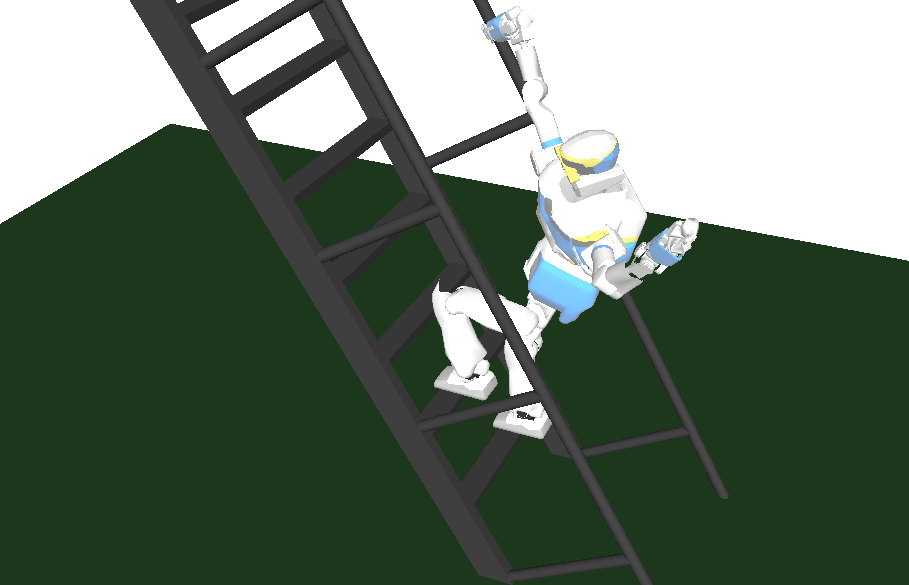
\includegraphics[width=\linewidth]{papers/IROS2014/figure/hrp2_ladder_darpa.png}}
%  %\fbox{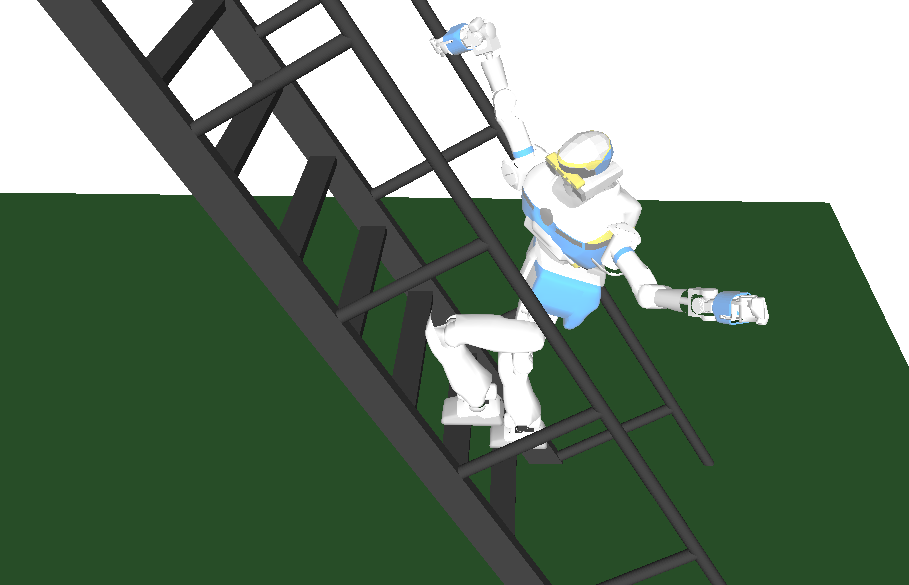
\includegraphics[width=\linewidth]{figure/hrp2_ladder_darpa_40.png}}
%  \fbox{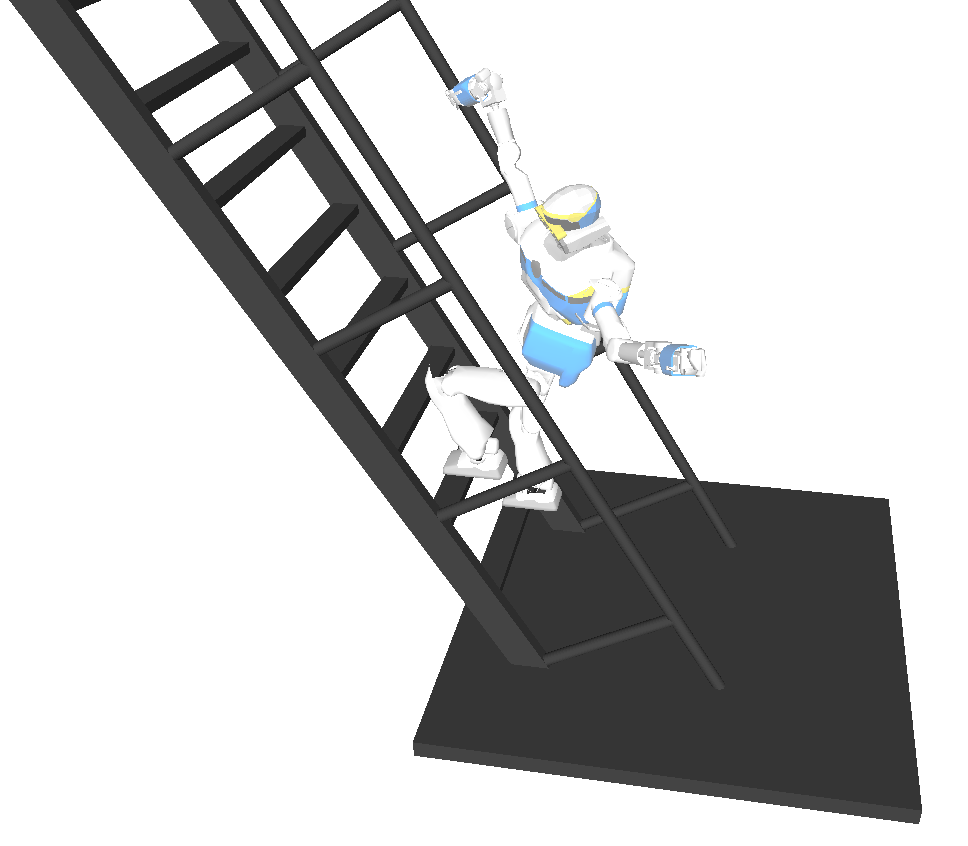
\includegraphics[width=\linewidth]{figure/hrp2_darpa_small.png}}
%  %\caption{HRP2-10 ladder climbing posture}
%  \label{fig:hrp2_darpa}
%\end{subfigure}%
%\begin{subfigure}{.5\textwidth}
%  \centering
%  \setlength\fboxsep{0pt}
%  \setlength\fboxrule{1pt}
%  %\fbox{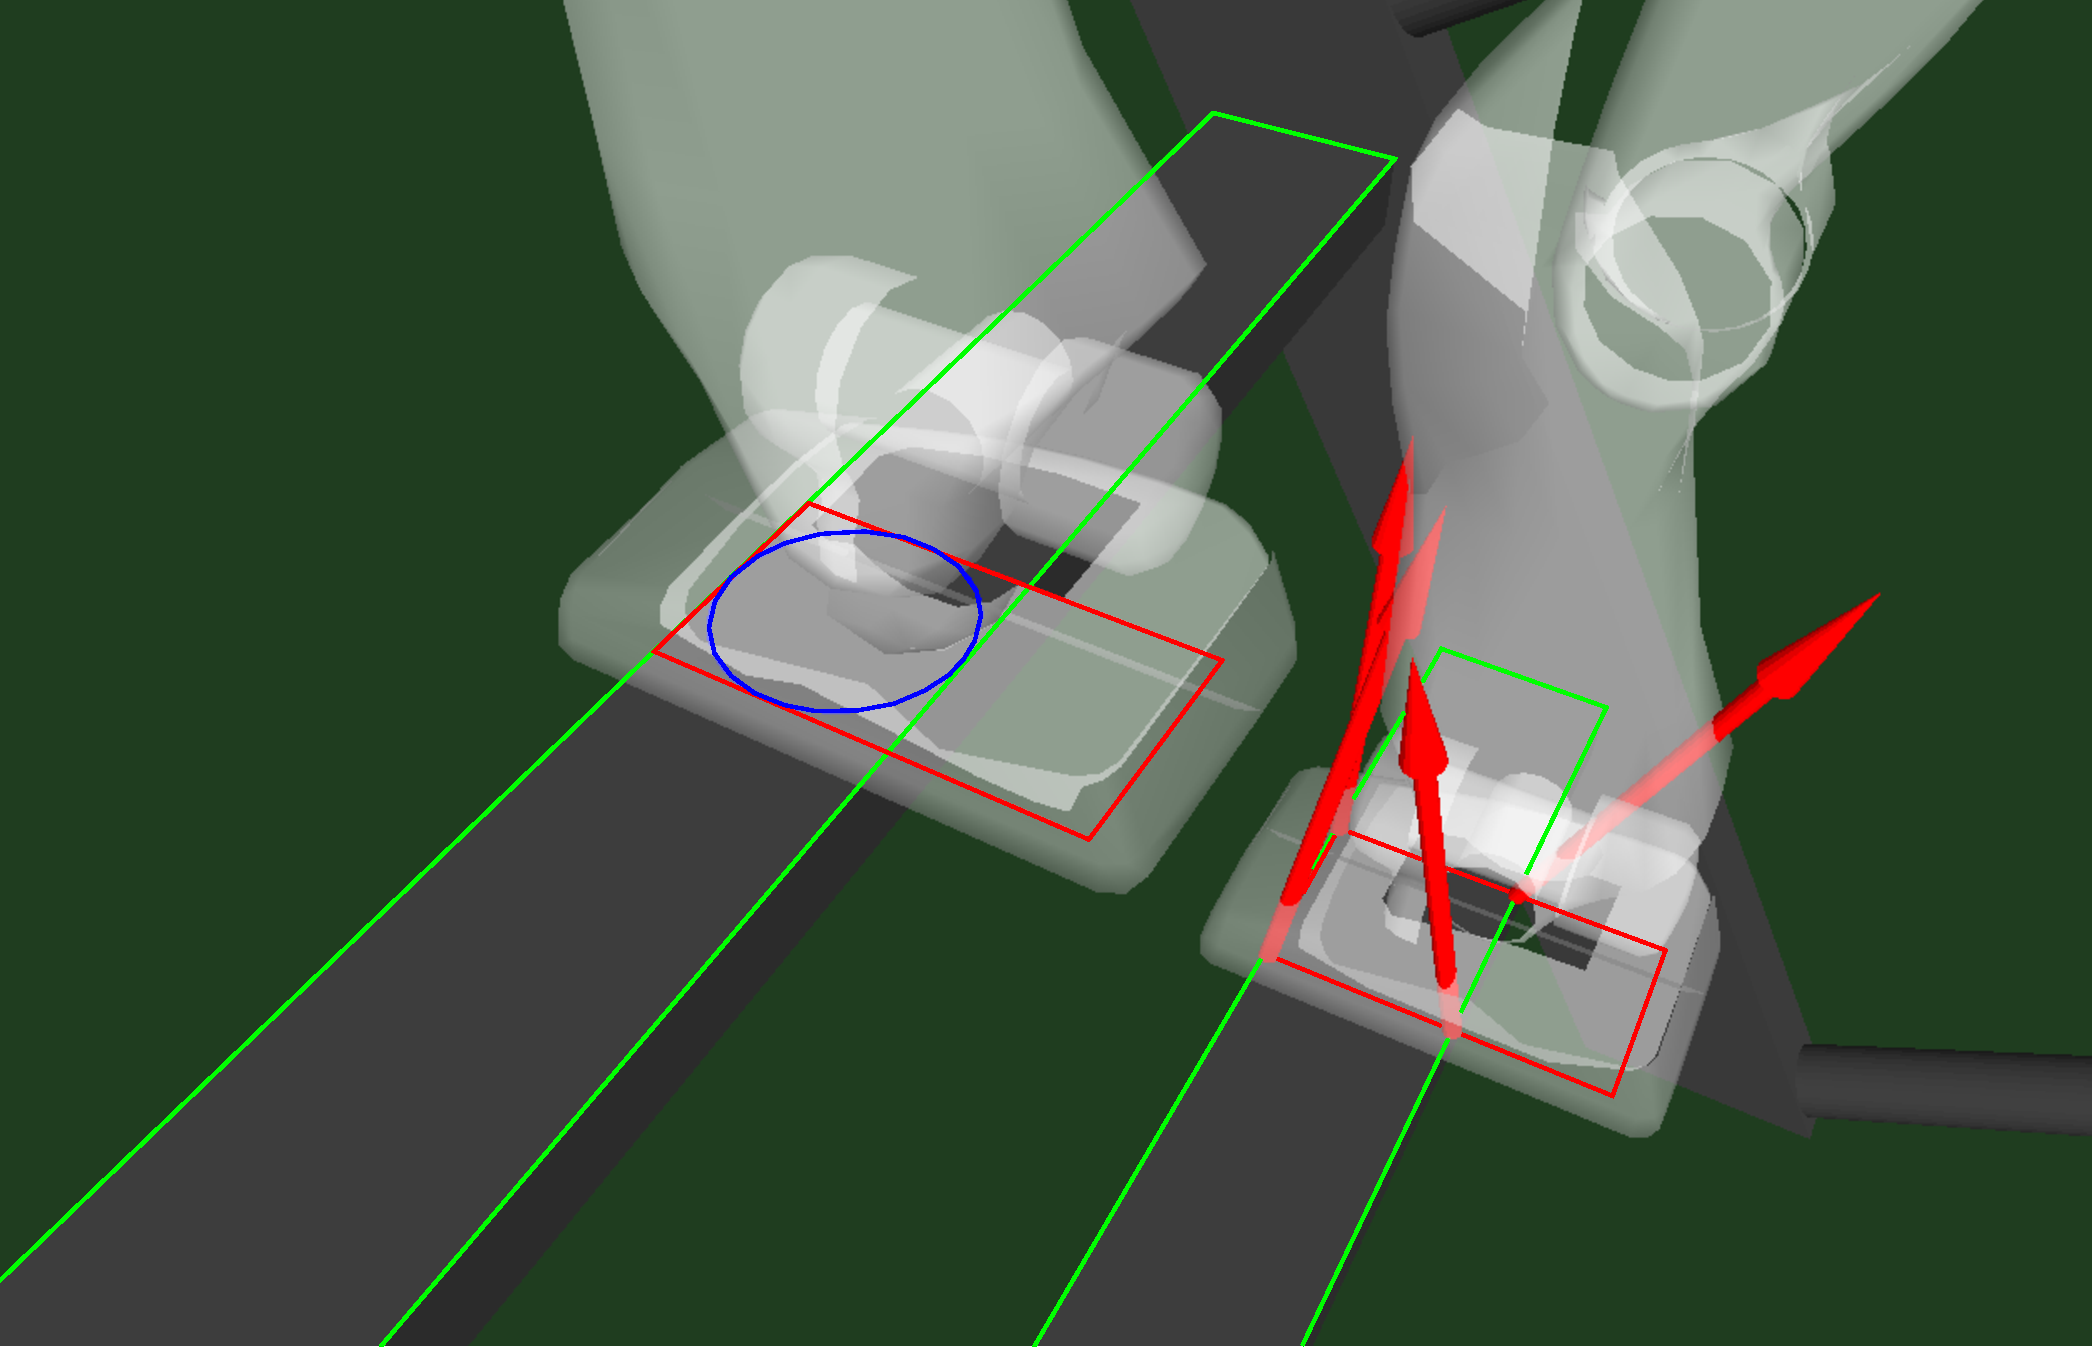
\includegraphics[width=\linewidth]{figure/hrp2_ladder_darpa_zoom.pdf}}
%  %\fbox{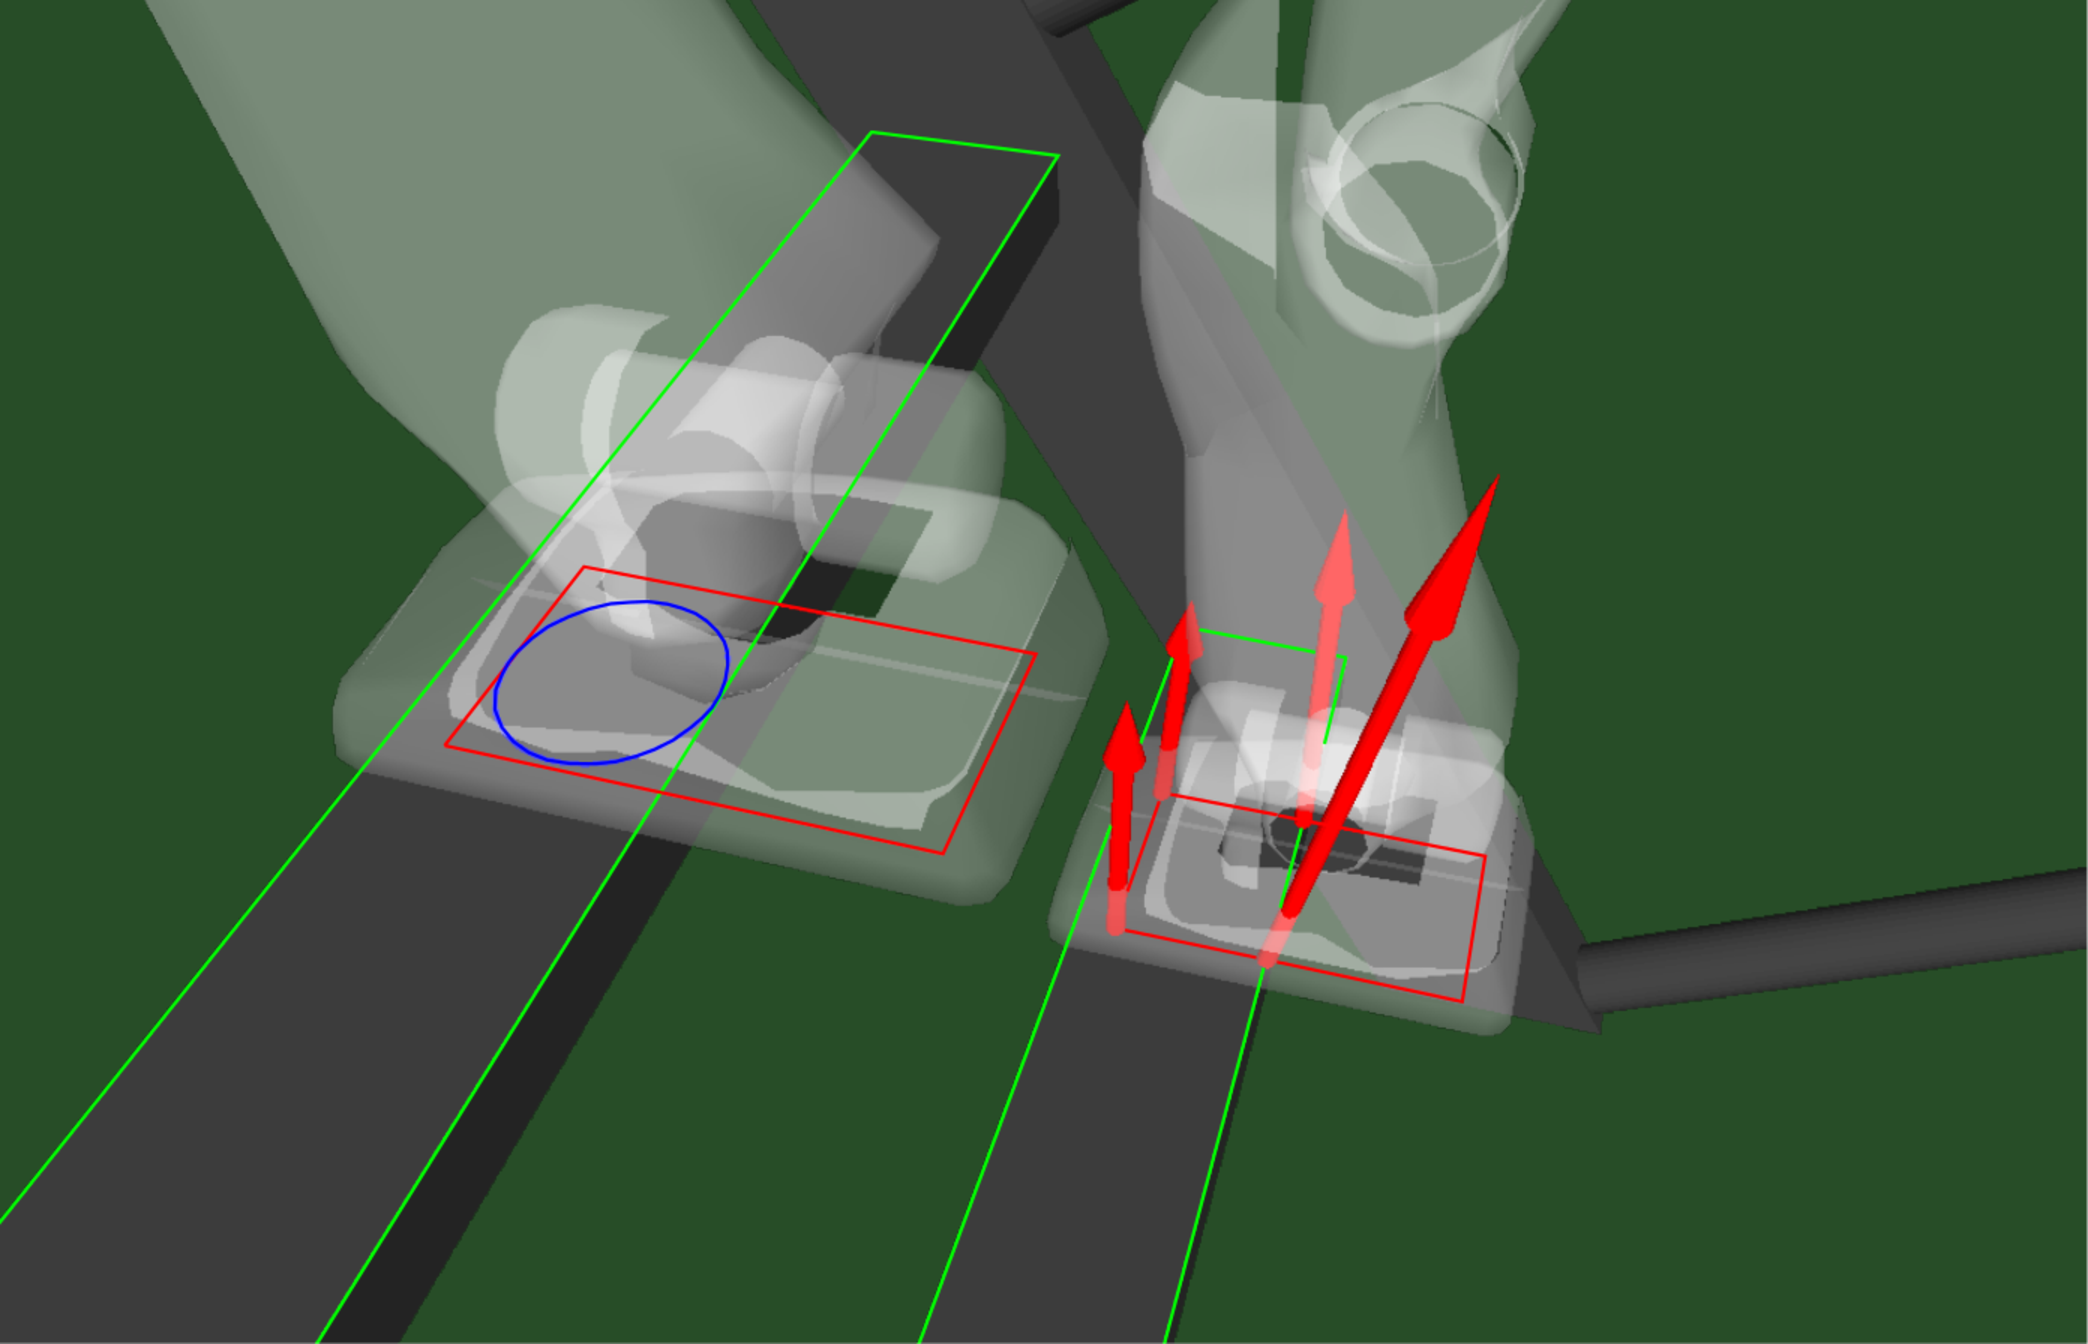
\includegraphics[width=\linewidth]{figure/hrp2_ladder_darpa_40_zoom.pdf}}
%  \fbox{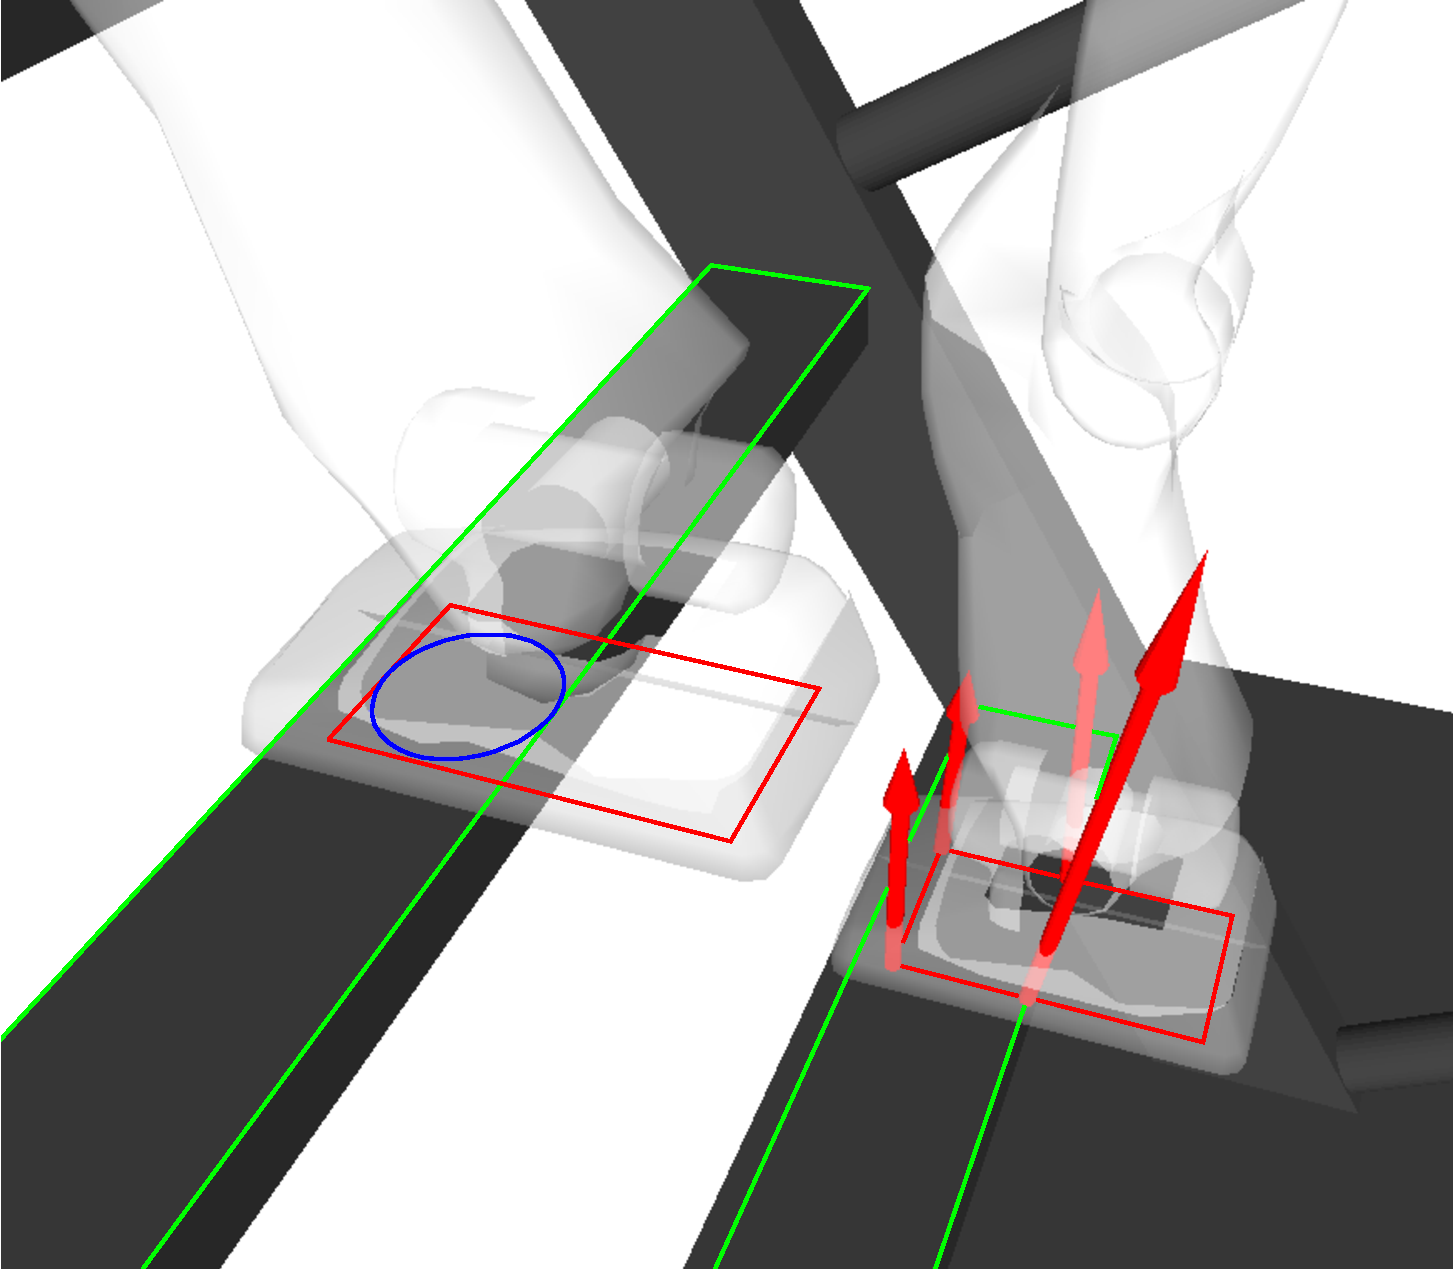
\includegraphics[width=\linewidth]{figure/hrp2_darpa_small_zoom.pdf}}
%  %\caption{Upclose view of the contact areas (green and red: contact polygon, blue: ellipse found in contact area, Red arrows: contact forces resultants)}
%  \label{fig:hrp2_darpa_zoom}
%\end{subfigure}
%\caption{(a)HRP2-10 ladder climbing posture; (b)Upclose view of the contact areas\\(green/red: contact polygons; blue: ellipse found in contact area; red arrows: contact forces resultants)}
%\label{fig:hrp2_darpa_complete}
%\end{figure*}  
\begin{figure}
\centering
\begin{subfigure}{.3325\columnwidth}
  \centering
  \setlength\fboxsep{0pt}
  \setlength\fboxrule{1pt}
  \fbox{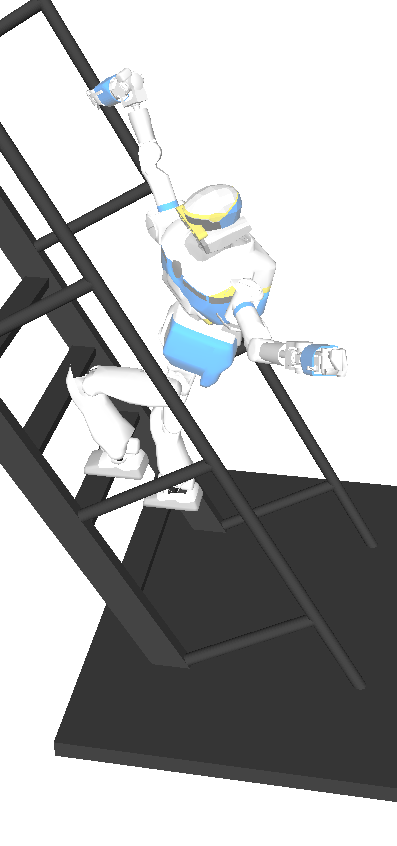
\includegraphics[width=\linewidth]{papers/IROS2014/figure/hrp2_darpa_small_cut.png}}
  \label{fig:hrp2_darpa}
\end{subfigure}%
\begin{subfigure}{.6175\columnwidth}
  \centering
  \setlength\fboxsep{0pt}
  \setlength\fboxrule{1pt}
  \fbox{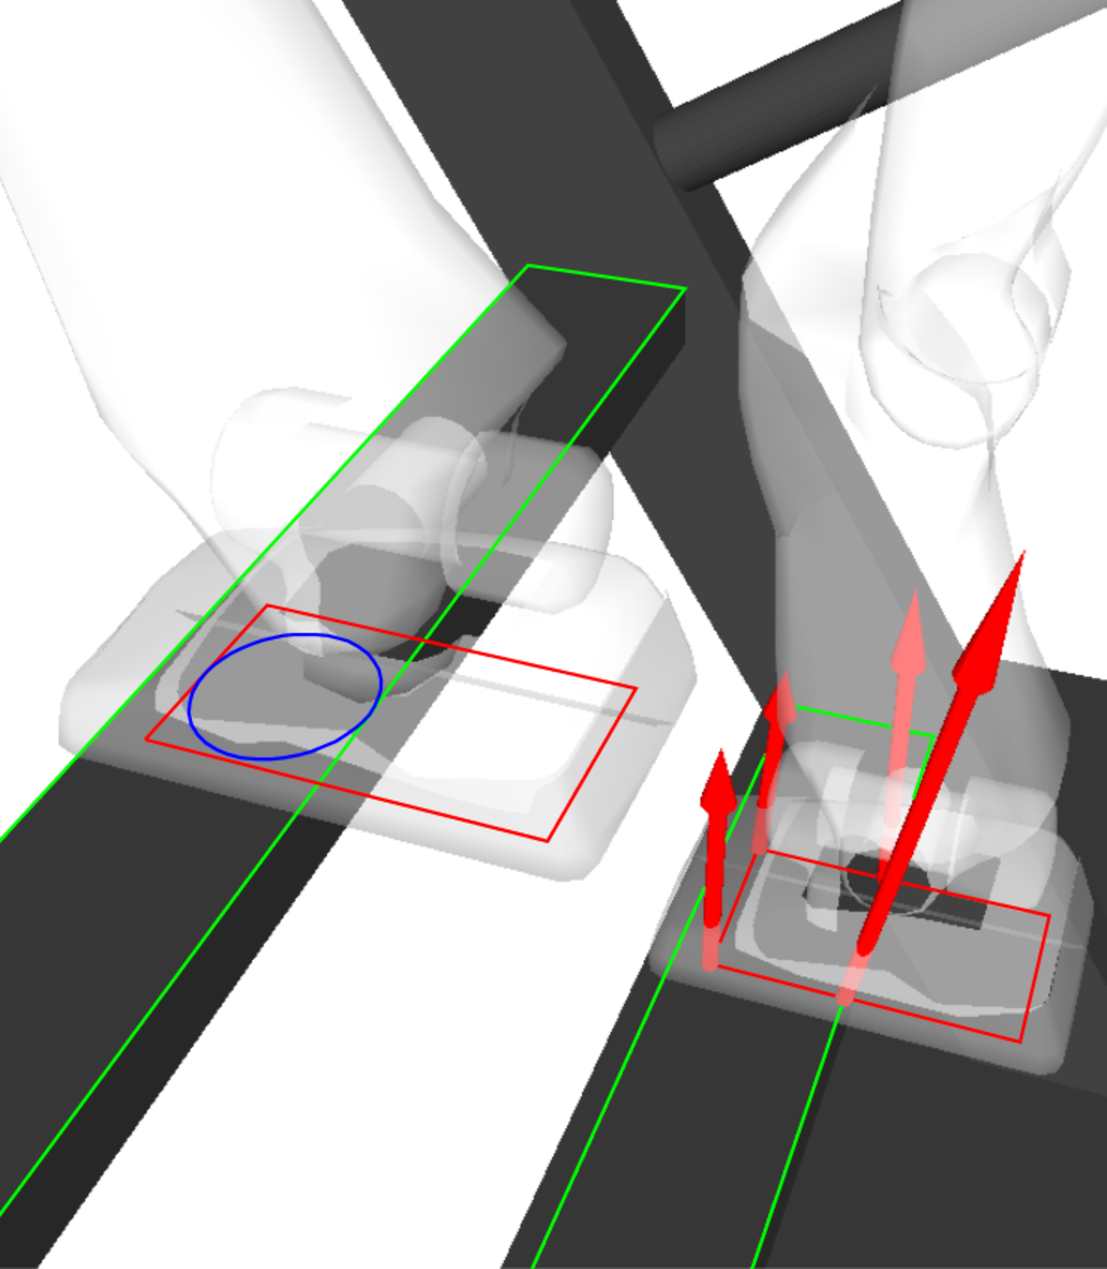
\includegraphics[width=\linewidth]{papers/IROS2014/figure/hrp2_darpa_small_zoom_cut.pdf}}
  \label{fig:hrp2_darpa_zoom}
\end{subfigure}
\caption{HRP2-10 ladder climbing posture and up close view of the contact areas (green/red: contact polygons; blue: contact ellipse; red arrows: contact forces resultants)}
\label{fig:hrp2_darpa_complete}
\end{figure}

\begin{figure*}
\centering
\setlength\fboxsep{0pt}
\setlength\fboxrule{1pt}
\fbox{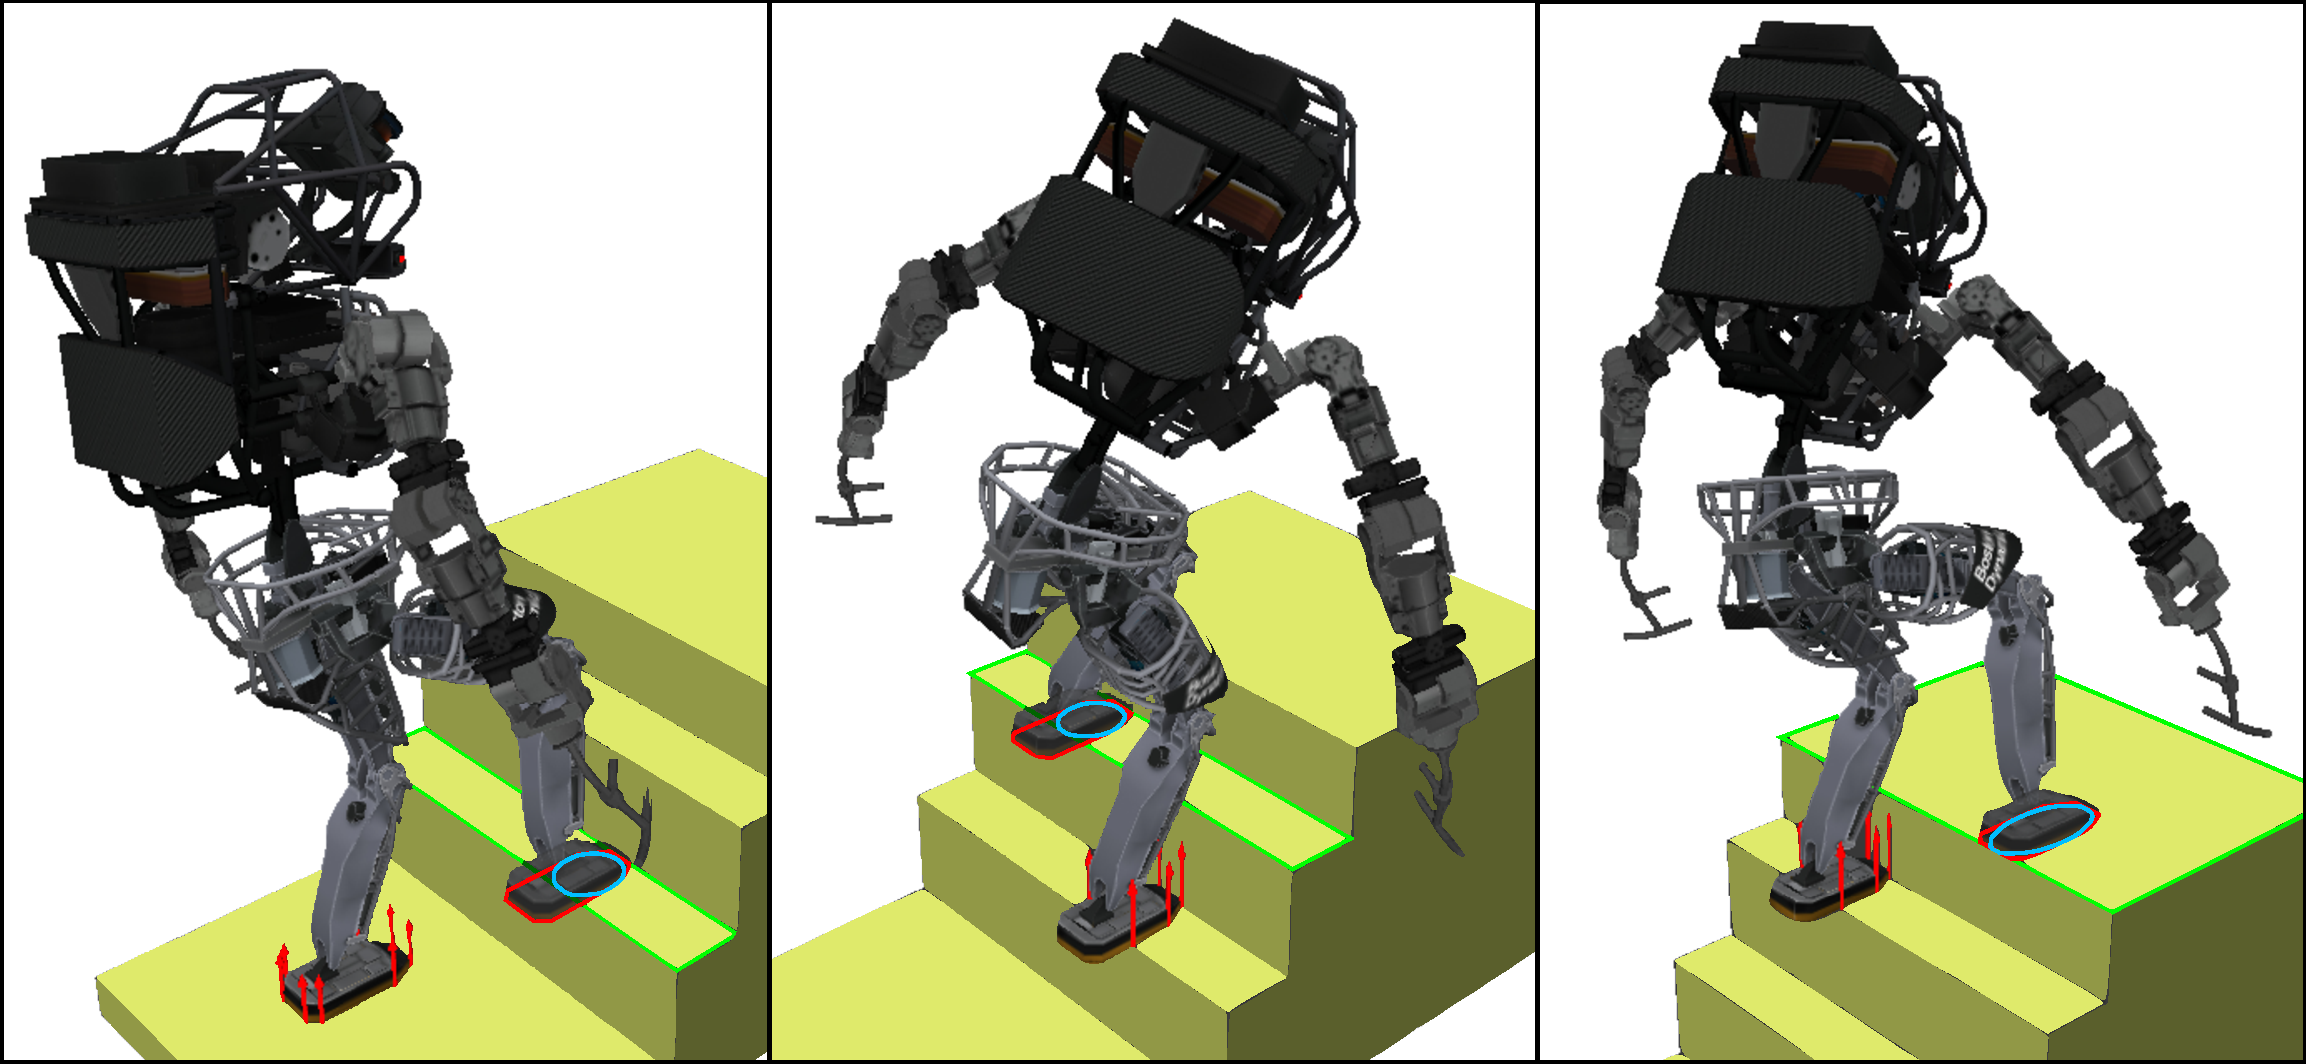
\includegraphics[width=0.95\linewidth]{papers/IROS2014/figure/atlas_1_2_3_yellow.pdf}}
\caption{Atlas climbing stairs with small steps by maximizing the size of the contact areas\\(green/red: contact polygons; blue: contact ellipse; red arrows: contact forces resultants)}
\label{fig:atlas_SmallStairs}
\end{figure*}  

\subsection{Vertical ladder climbing}
\label{subsec:ladder}

In the second example we generate a posture in which the robot climbs a vertical ladder.
In this particular step, the robot is using its right foot and both hands to maintain its stability on top of the first rung of the ladder. We search a posture that keeps those previous contacts and adds a geometrical contact between the left foot and the second rung of the ladder.
The result of that optimization can be observed on ~\Figref{fig:hrp2_jrl_complete}, with the robot posture on the left and a close-up look at the contact areas on the right.
The difficulty of this situation is that a contact has to be made with a very thin surface of the environment (the ladder rung). Usual contact generation method would reduce a lot the span of possible contact position (by patching the robot's foot with a very small surface or by imposing a set of authorized contact positions).
Whereas with our method, the contact configuration is found during the optimization process without requiring any extra human work. The contact chosen by our software includes an ellipse which first axis is the width of the robot's foot and second axis is as thin as the ladder rung.   
One problem to expect is that numerical instability might happen if the surface of the rung is given too thin. But that would also happen with full inclusion constraints.
This example also illustrates one limitation of our method: it only considers planar contacts and if one wants to model a purely linear contact an other contact model must be used, since our modeling of those singular cases is approximative.
%is the first step of the HRP-2 robot climbing a ladder. The two hands are in bilateral contact with the two side bars of the ladder, the left foot is fixed on the ground and is the only part of the robot involved in the stability. The right foot is to make a contact with the first rung of the ladder. The rungs of the ladder are modeled by rectangles with a 6mm width which approximates the contact line as explained in section~\ref{subsec:singular cases}. %Therefore, the ellipse area maximization takes place in the intersection of the polygons representing the rung and the foot. 
%The result of that optimization can be observed on ~\Figref{fig:ladder}{}.
%On the right of the simulation image is shown the disposition of the foot (in green) that is in geometrical non inclusive contact with a rung (in blue) and the optimal ellipse that has been found.


%From a planning point of view, this particular result is obviously not achievable as the right leg of the robot goes through the ladder, this will be discussed in the next section. Yet, the posture is perfectly valid as it respects of the constraints of problem~(\ref{eq:PG}). This example illustrates our method in a multi-contact environment with almost linear contacts. 
%

\subsection{Climbing Stairs}
\label{subsec:smallStairs}

In a third simulation, the ATLAS robot climbs a flight of stairs.
All the steps are too small for the robot to put its entire foot on.
Therefore, it has to make a non inclusive contact and we propose to maximize the size of the contact area with the ellipse included in it, as explained in \ref{subsec:optim-ellipse-area}. 
The size of the contact area is limited by the fact that the foot cannot penetrate the wall behind each step.
On~\Figref{fig:atlas_SmallStairs}, we present 3 postures generated on this environment.
On each of those postures, we see that the ellipse's size is maximized until the foot enters in collision with the vertical wall behind each step. And when possible, like on the last step, the contact area is maximized without collision limitation and the foot is positioned as fully included in the support surface.
We can see here that even when the size of the ellipse is maximized while competing with other non-linear constraints like collision avoidance, our method still works well and leads us to a satisfactory solution.

%Under each simulation result, an image presents the disposition of the foot (in green) that is in geometrical non inclusive contact with a step (in blue) and the optimal ellipse that has been found.
%It has to be noted that the green contact surface under a foot of the robot (green rectangle) is actually smaller than the actual foot due to our use of security margin for stability reason when experimenting with real robot and take into account an un-modeled flexibility at the ankle.
%That is why, with the collision avoidance activated between the foot and the next step, it seems that the foot is still far from the limit of the step (blue rectangle).
%Actually the foot is almost in collision with the vertical part of the next step.
%We decided not to present the initial and final steps of this hypothetical movement because they do not bear any interesting aspect as they both consist of the robot standing on a large flat surface.

%\begin{figure*}
%\centering
%\begin{subfigure}{.319\textwidth}
%  \centering
%  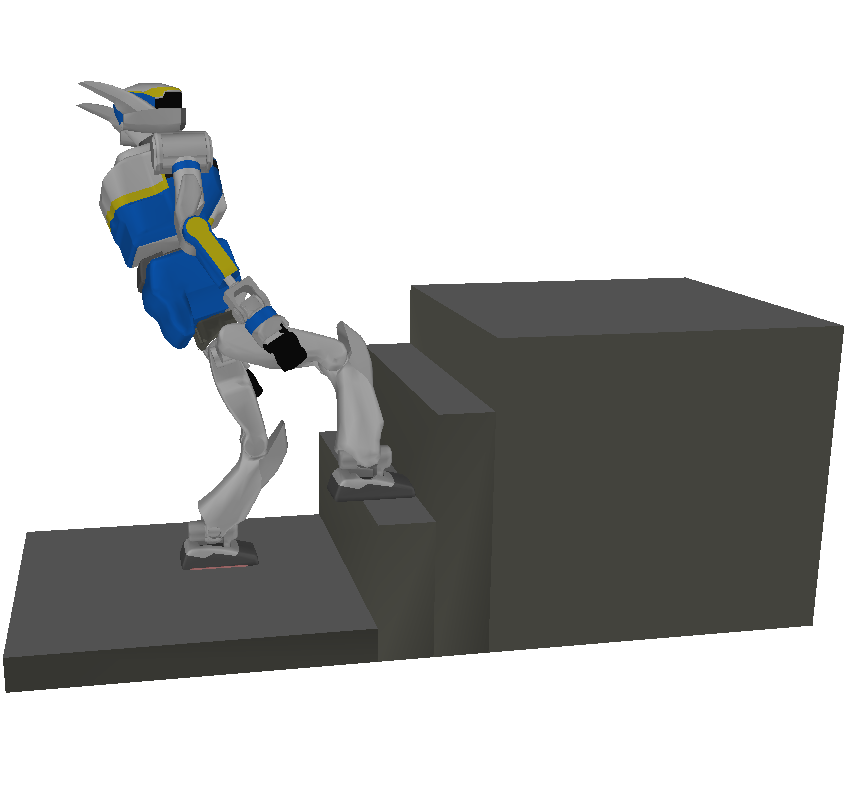
\includegraphics[width=\linewidth]{figure/SmallStairs2.png}
%\end{subfigure}%
%\begin{subfigure}{.3\textwidth}
%  \centering
%  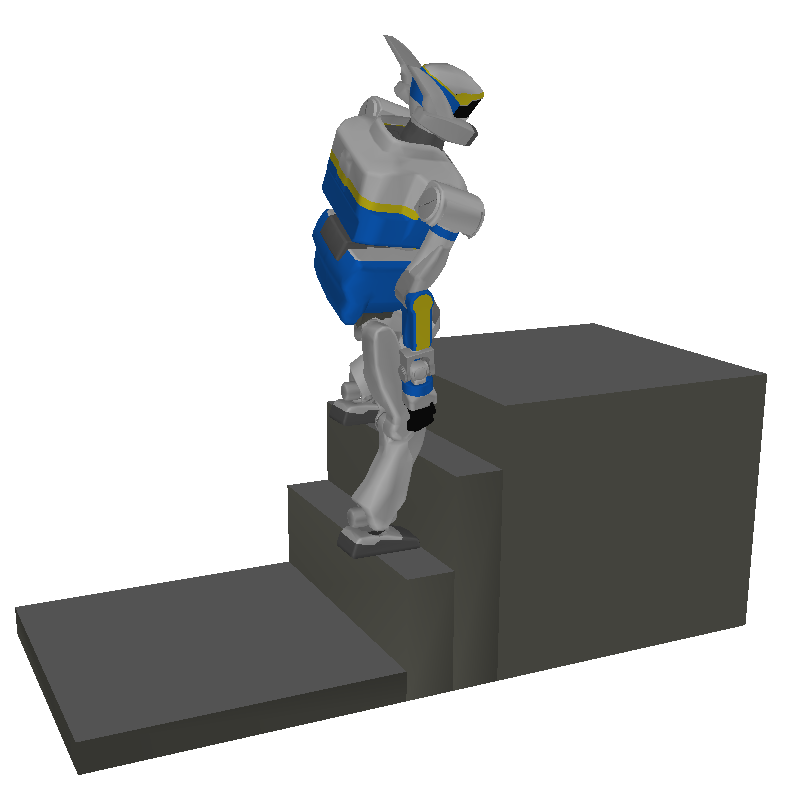
\includegraphics[width=\linewidth]{figure/SmallStairs3.png}
%\end{subfigure}
%\begin{subfigure}{.3\textwidth}
%  \centering
%  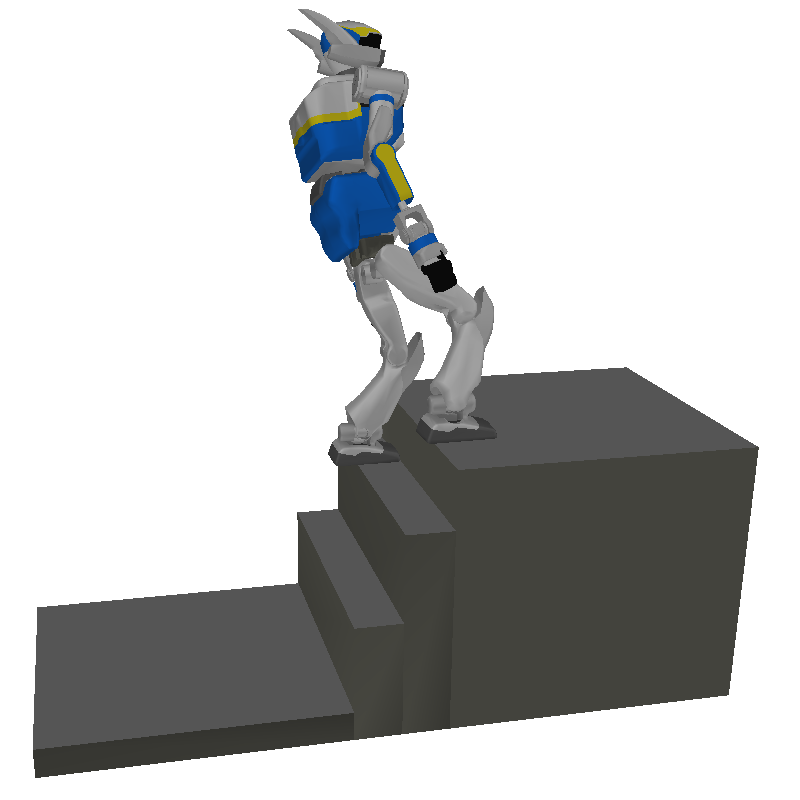
\includegraphics[width=\linewidth]{figure/SmallStairs4.png}
%\end{subfigure}
%\caption{Using non-inclusive contacts for ladder climbing}
%\label{fig:hrp2_SmallStairs}
%\end{figure*}  

%\subsection{Walking along a path made of small objects}
%
%In the second simulation, the HRP-2 robot has to cross a gap by making contacts
%with small surfaces. As well as for the previous simulation, the two objects
%with which the feet of the robot will be in contact are too small for making a
%complete contact, instead, non inclusive geometric contacts are found by
%maximizing the area of an ellipse that fits in the intersection of the polygons
%involved in the contact. Results are presented in ~\Figref{fig:riviere}. As
%we can see, the feet turns slightly, to be more aligned with the support
%surfaces, yet they do not become completely aligned with these supports, which would permit to get the biggest ellipse area. This is due to the fact that a posture cost is competing with the area cost, yielding this compromise.
%%Under each simulation result, an image presents the disposition of the foot (in green) that is in geometrical non inclusive contact with a step (in blue) and the optimal ellipse that has been found. We decided not to present the initial and final steps of this hypothetical movement because they do not bear any interesting aspect as they both consist of the robot standing on a large flat surface.
%
%\label{subsec:riviere}
%\begin{figure*}[!htb]
% \centering
% 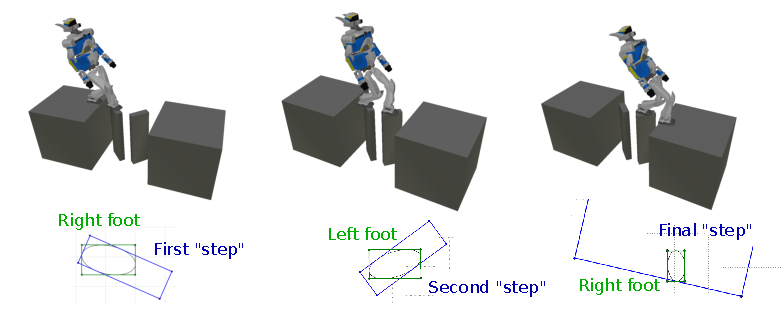
\includegraphics[width=0.75\textwidth]{figure/riviere3steps.pdf}
% \caption{Simulation results for crossing a gap by walking on small items}
% \label{fig:riviere}
%\end{figure*}
%
\section{Discussion and conclusion}
Generating arbitrary shaped contact areas proved to be doable very simply in an optimization-based posture generation module. We focused on writing constraints that have continuous gradients, since the posture generate problem is dominantly smooth. Hence, our geometric contact model can be useful for other optimization-based purposes, for example control or trajectory optimization, and any gradient-based descent scheme which handles inequalities (e.g.~\cite{escande:icra:2010}).
While we were expecting an increase of computation time due to the addition of new variables in the problem,
% (5 more for a total of 80-100 variables)
we noticed that the timings obtained with this method are sensibly the same that our previous version of the posture generator with full contact surface inclusion. Consequently, this method offering a richer contact search (exploration) during planning comes without degrading computation time. In fact, it truly allows us to substantially reduce the time spent by the user in ad-hoc tuning the shapes of the contact patches, or fixing the contact positions that were previously done by hand. Also, it is fairly easy to implement and extends a multi-contact planning algorithms like the one described in~\cite{escande:ras:2013}{} to give it richer planning possibilities.

There are several opportunities for future work. For example, we could improve the generality of our contact constraint formulation even further to manage linear and punctual contacts without the approximations we currently use. Also we could extend our method to allow dealing with non-convex surfaces. And finally we would like to apply our method to other fields that use contact generation, like trajectory or control optimization. Our methods extends straightforwardly to point cloud data as far as polygonal patches can be extracted.
%While we were expecting an increase of computation time due to the addition of new variables in the problem (5 more for a total of 80-100 variables), we were surprised by the obtained timings, around $10s$ while a usual posture generation is less than $1s$. Part of this increase is obviously due to the fact that we used finite differences to compute the gradients of the new constraints and objectives, and one of the immediate on-going works is to derive and implement efficiently analytical gradients. Still, we will also investigate more thoroughly how the new constraints interact with the existing ones to look for potential other causes for this increase.

%Finally, on a planning point of view, ~\Figref{fig:ladder} shows us a new challenge: while the posture found is perfectly correct as the robot is stable, not colliding with its environment and the contacts are where we asked them to be, the posture is obviously difficult to attain, if possible at all. We will need to investigate what type of heuristic to use to avoid this kind of results in the middle of a plan.
